\chapter[Identificación de Métodos Generadores de Objetos]{Identificación de Métodos Generadores de Objetos}
\label{cap:builders}

\cacho{1 - terminar las citas}

% Primera etapa
\section{Ejemplo Motivador}

\begin{table}[]
\centering
{\scriptsize
\begin{tabular}{|l|l|l|}
\hline
No. & Nombre del Método & Observador? \\
\hline
0 & NCL() & no \\
1 & NCL(int) & no \\
2 & NCL(Collection) & no \\
3 & add(Object) & no \\
4 & add(int,Object) & no \\
5 & addAll(Collection) & no \\
6 & addAll(int,Collection) & no \\
7 & addFirst(Object) & no \\
8 & addLast(Object) & no \\
9 & clear() & no \\
10 & contains(Object) & sí \\
11 & containsAll(Collection) & sí \\
12 & equals(Object) & sí \\
13 & get(int) & sí \\
14 & getFirst() & sí \\
15 & getLast() & sí \\
16 & indexOf(Object) & sí \\
17 & isEmpty() & sí \\
18 & iterator() & no \\
19 & lastIndexOf(Object) & sí \\
20 & listIterator() & no \\
21 & listIterator(int) & no \\
22 & remove(int) & no \\
23 & remove(Object) & no \\
24 & removeAll(Collection) & no \\
25 & removeFirst() & no \\
26 & removeLast() & no \\
27 & retainAll(Collection) & no \\
28 & set(int,Object) & no \\
29 & size() & sí \\
30 & subList(int,int) & si \\
31 & toArray() & sí \\
32 & toArray(Object[]) & sí \\
33 & toString() & sí \\
\hline
\end{tabular}
}
\caption{API de NodeCachingLinkedList de Apache}
\label{tab:ncl-api}
\end{table}


Para comprender mejor la definición de métodos generadores de objetos, motivaremos la misma mediante un ejemplo de una API real. La estructura de datos NodeCachingLinkedList (NCL) de Apache \cite{apache} está diseñada como una lista principal, circular y doblemente enlazada, que almacena los elementos de la colección. Además, incluye una lista secundaria simplemente enlazada que actúa como caché para nodos eliminados de la lista principal. Esta caché permite reutilizar los nodos almacenados, mejorando el rendimiento en aplicaciones donde las operaciones de inserción y eliminación son frecuentes. Gracias a esta optimización, NCL reduce significativamente la sobrecarga asociada a la asignación de memoria y a la recolección de basura. 

La API de NodeCachingLinkedList incluye un conjunto de métodos (ver tabla \ref{tab:ncl-api}) que permiten construir, modificar y consultar la colección. Esta API combina funcionalidades típicas de listas enlazadas con optimizaciones adicionales relacionadas con el reuso de nodos en la caché. Los métodos pueden clasificarse en tres categorías principales según su función: 

\begin{itemize}
    \item \textbf{Métodos constructores:}
    Los métodos constructores (líneas 0-2 en la Tabla~\ref{tab:ncl-api}) permiten crear nuevos objetos del tipo. Estos son:
    \begin{itemize}
        \item \texttt{NCL()}: Crea una lista vacía.
        \item \texttt{NCL(int)}: Crea una lista vacía. El parámetro define el
            tamaño máximo permitido para la lista caché.
        \item \texttt{NCL(Collection)}: Crea una lista nueva que contiene todos los elementos de una colección dada.
    \end{itemize}
    \item \textbf{Métodos modificadores:}
    Estos métodos permiten agregar, eliminar o modificar elementos de la lista. Algunos ejemplos son:
    \begin{itemize}
        \item \texttt{add(Object)}: Agrega un elemento al final de la lista
            principal. \cacho{Si hay nodos disponibles en la lista cache, se reutiliza uno de ellos.}\pp{No puede ser,
            la cache estaría al pedo si fuera así porque no se reusan los nodos. Revisar}
        \item \texttt{addFirst(Object)} y \texttt{addLast(Object)}: Insertan elementos al principio o al final de la lista principal 
        \cacho{En ambos casos, si existen nodos disponibles en la cache, se reutilizan para evitar la creación de nuevos nodos.}\pp{No puede ser,
            la cache estaría al pedo si fuera así porque no se reusan los nodos. Revisar}
        \item \texttt{remove(int)} y \texttt{remove(Object)}: Eliminan elementos de la lista por índice o por valor. El nodo eliminado se inserta en la lista cache de la estructura.
        \item \texttt{clear()}: Vacía la lista principal y se insertan los nodos
            eliminados en la lista cache.
        \item \texttt{set(int, Object)}: Modifica el elemento en una posición específica de la lista.
    \end{itemize}
    \item \textbf{Métodos observadores:}  
    Estos métodos permiten inspeccionar el estado de la lista sin modificarla:
    \begin{itemize}
        \item \texttt{contains(Object)}: Verifica si un elemento está presente.
        \item \texttt{get(int)}, \texttt{getFirst()} y \texttt{getLast()}: Recuperan elementos según su posición.
        \item \texttt{size()}: Retorna el número de elementos en la lista.
        \item \texttt{toArray()}: Crea un nuevo arreglo con todos los elementos de la lista.
    \end{itemize}
\end{itemize}

\noindent
A partir de esta API, los objetos de \emph{NodeCachingLinkedList} pueden
construirse utilizando secuencias de operaciones que combinan los métodos
constructores y los modificadores. Por ejemplo, una lista inicializada con
\texttt{NCL()} puede llenarse mediante llamados consecutivos a
\texttt{add(Object)} o \texttt{addAll(Collection)}, mientras que los métodos
\texttt{remove(Object)} y \texttt{clear()} permiten mover nodos de la lista
principal a la lista cache.

La Figura~\ref{fig:ncl-instances-intro} muestra tres instancias de NodeCachingLinkedList. A continuación, se presentan las secuencias de métodos generadores que permiten construir cada una de las configuraciones:

\begin{figure}[H]
    \centering
    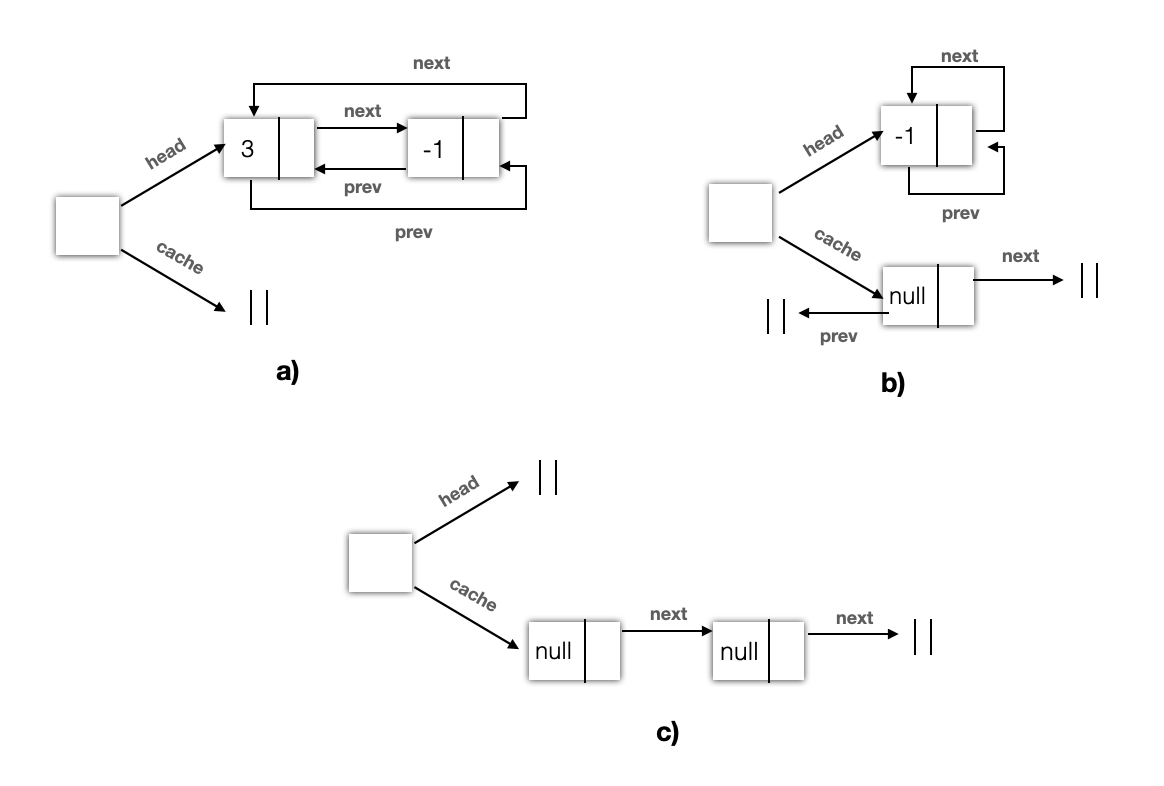
\includegraphics[width=1.0\textwidth]{images/ncl_instancias.png}
    \caption{Tres instancias de NodeCachingLinkedList con exactamente dos nodos.}
    \label{fig:ncl-instances-intro}
\end{figure}

\begin{itemize}
\item Figura (a): Esta instancia se construye agregando dos elementos a la lista
    principal, por ejemplo, ejecutando la siguiente secuencia de test:
\vspace{5pt} 
    \begin{lstlisting}[numbers=none,label=fig:NCLbuilders_a,xleftmargin=0pt]
    (0)  NodeCachingLinkedList();
    (7)  addFirst(3);
    (7)  addFirst(-1);
    \end{lstlisting}

\item Figura (b):
    \cacho{Esta instancia se logra agregando dos nodos a la lista principal y luego eliminar uno de ellos. En este caso el primero en agregar a la lista principal
    y se mueve el nodo a la lista cache}
    \vspace{5pt} 

    \begin{lstlisting}[numbers=none,label=fig:NCLbuilders_b, xleftmargin=0pt]
    (0)  NodeCachingLinkedList();
    (7)  addFirst(3);
    (7)  addFirst(-1);
    (25) removeFirst();
    \end{lstlisting}

\item Figura (c): 
    Esta instancia se genera añadiendo dos nodos al inicio y luego eliminándolos
    para pasarlos a la lista cache
    \vspace{5pt} 

    \begin{lstlisting}[numbers=none,label=fig:NCLbuilders_c, xleftmargin=0pt]
    (0)  NodeCachingLinkedList();
    (7)  addFirst(3); 
    (7)  addFirst(-11); 
    (25) removeFirst();
    (25) removeFirst();
    \end{lstlisting}
\end{itemize}



\section{Métodos Generadores de Objetos y sus Propiedades}

%\pp{Definición de generadores de objetos}
Se puede observar que, a pesar de que la API de NCL es muy compleja, como se observa en la Tabla~\ref{tab:ncl-api}, no todos los métodos son necesarios para construir objetos. 
Por ejemplo, combinaciones de los métodos mostrados en la Figura~\ref{fig:NCLbuilders}, con los parámetros adecuados, son suficientes para generar cualquier instancia de NCL.
\vspace{5pt} 
\begin{lstlisting}[numbers=none,label=fig:NCLbuilders, caption=Conjunto de métodos generadores de objetos para NCL]
  (0)  NodeCachingLinkedList()
  (7)  addFirst(Object)
  (25) removeFirst()
\end{lstlisting}

Una vez inicializada la instancia de NCL con el constructor, se pueden insertar elementos en la lista utilizando el método \texttt{addFirst}. Adicionalmente, el método \texttt{removeFirst} permite crear instancias que posean nodos en la lista caché (eliminando el nodo de la lista principal). 

De esta manera, los métodos de la Figura~\ref{fig:NCLbuilders} conforman un conjunto \emph{suficiente de métodos generadores de objetos}, es decir, son conjuntos de métodos que permiten generar todos los objetos posibles de NCL. Por simplicidad, llamaremos \emph{generadores de objetos} a estos métodos.

Notar que pueden existir distintos subconjuntos suficientes de generadores de objetos, como por ejemplo los que se muestran en las Figuras~\ref{fig:NCLbuilders2} y~\ref{fig:NCLnoMin1}. 
\vspace{5pt} 
\begin{lstlisting}[numbers=none,label=fig:NCLbuilders2, caption=Otros métodos generadores de objetos, frame=tb , basicstyle=\scriptsize, xleftmargin=0pt]
  (0)  NodeCachingLinkedList()
  (3)  add(Object)
  (25) removeFirst()
\end{lstlisting}


En particular, la Figura~\ref{fig:NCLnoMin1} contiene métodos \emph{superfluos}, es decir, métodos que pueden quitarse sin perder la propiedad de suficiencia del conjunto resultante. Por ejemplo, podemos eliminar \texttt{remove(Object)} y los métodos restantes siguen siendo generadores de objetos suficientes (similarmente, podríamos eliminar \texttt{removeFirst()}). 
\vspace{5pt} 

\begin{lstlisting}[numbers=none,label=fig:NCLnoMin1, caption=Métodos generadores de objetos suficientes pero no minimales, captionpos=b, frame=tb , xleftmargin=0pt, basicstyle=\scriptsize]
  (0)  NodeCachingLinkedList()
  (7)  addFirst(Object)
  (3)  remove(Object)
  (25) removeFirst()
\end{lstlisting}

Estamos interesados en conjuntos de métodos generadores de objetos \emph{minimales}, es decir, en conjuntos generadores de objetos suficientes con la menor cantidad posible de métodos. En otras palabras, los generadores de objetos son minimales si la exclusión de cualquiera de los métodos hace imposible la creación de ciertas instancias del módulo.
Así, las Figuras~\ref{fig:NCLbuilders} y ~\ref{fig:NCLbuilders2} muestran ejemplos de generadores de objetos suficientes y minimales.

Notar que muchos métodos en la tabla \ref{tab:ncl-api} están marcados como observadores (columna Obs?), lo que significa que no modifican los objetos sobre los que operan, ni son útiles para crear nuevos objetos. 
Debido a que estos métodos observadores siempre son superfluos y nunca deben incluirse en un conjunto de generadores de objetos minimal. Por esta razón, nuestros enfoques de identificación de métodos generadores intentan reconocerlos de antemano y descartarlos.

Por último, observamos que cuanto más fáciles de instanciar sean los parámetros de una rutina, usualmente la rutina será más eficiente de utilizar en el contexto de un análisis de programas (por ejemplo, para generar entradas para testing). Por ejemplo, entre las alternativas de rutinas para insertar datos en
la lista principal de NCL (ver Tabla~\ref{tab:ncl-api}), \texttt{add(int,Object)} recibe más parámetros que los otros tres métodos posibles. En cambio, \texttt{add(Object)}, \texttt{addFirst(Object)}, \texttt{addLast(Object)} toman un único parámetro. Si bien cualquiera de estas rutinas sirve para generar los mismos objetos de NCL, hay más formas de invocar a \texttt{add(int,Object)}. Esto usualmente redunda en una pérdida de eficiencia en la construcción de objetos por parte de un análisis automático de programas. Similarmente, elegiremos métodos con parámetros más simples (por ejemplo, parámetros de tipo primitivo), que otros con parámetros más complejos (por ejemplo, parámetros de tipo referencia) siempre y cuando los métodos permitan construir los mismos objetos.

De la discusión anterior se desprende que preferimos los métodos con menor número de parámetros, y con parámetros más fáciles de instanciar en los generadores de objetos (siempre que se mantengan las propiedades de suficiencia y minimalidad de los generadores). 
En nuestro ejemplo anterior, elegiremos \texttt{add(Object)} (o \texttt{addFirst(Object)} o \texttt{addLast(Object)}) en lugar de \\
\texttt{add(int,Object)} 
como parte de un conjunto suficiente y minimal de generadores de objetos.

Para concluir esta sección, es importante destacar que identificar manualmente un conjunto suficiente y minimal de métodos generadores de objetos es una tarea difícil y trabajosa, que requiere inspeccionar minuciosamente el código fuente del módulo y las formas en las que los métodos interactúan entre sí para generar objetos. Esto se dificulta aún más cuando los módulos cuentan con APIs ricas, como en nuestro ejemplo motivador (ver Tabla~\ref{tab:ncl-api}). 
Para facilitar la tarea del desarrollador, en las secciones siguientes proponemos enfoques automáticos para identificar conjuntos de métodos generadores de objetos.

\pp{Quizás esto sirva para explicar la explosión de combinaciones de métodos en los análisis de programas? Hay que pensarlo..} 
\pp{Pablo: Builders usage in program analyses? Now or later? We'll see...}

\section{Definiciones preliminares}
\label{sec:preliminares}


% Intro
En este capítulo, nos enfrentamos al desafío de identificar un conjunto suficiente y mínimo de generadores de objetos a partir de la API de un módulo. 
Nos enfrentamos a un problema de optimización, donde apuntamos a encontrar el mejor estado según una función objetivo.
Esta definición es la de los algoritmos de búsqueda local \cite{Russell:2009}.
Para abordar este problema desarrollamos dos algoritmos de búsqueda, cada uno con su enfoque único. Estos algoritmos nos permiten explorar el espacio de búsqueda de manera eficiente y efectiva.

El primer algoritmo que presentamos es un enfoque basado en algoritmos genéticos, que utiliza principios inspirados en la evolución biológica \cite{Goldberg:1989}
%, este algoritmo se enfoca en generar conjuntos de métodos generadores que puedan dar lugar a configuraciones más grandes y diversas de objetos. 
La naturaleza basada en la evolución de este enfoque permite encontrar soluciones prometedoras y adaptarse a diferentes situaciones.

El segundo algoritmo que proponemos es un enfoque \emph{greedy}, específicamente una variante de un algoritmo de ascenso de colinas \cite{Russell:2009,Cormen2009}. Este enfoque se centra en mejorar iterativamente un conjunto inicial de métodos generadores mediante la adición de métodos.
%, buscando siempre mejorar la calidad del conjunto en términos de eficiencia en cuanto a los objectos generados y la cobertura que se logra utilizando estos objectos sobre la API bajo test.

%Por último, presentamos un algoritmo basado en la idea de particionar los subconjuntos de métodos de la API en "clases de equivalencias" según los objetos que construyen. Esta estrategia nos permite agrupar métodos con propiedades similares y seleccionar conjuntos de métodos más cohesivos y efectivos.

Cada uno de estos algoritmos ofrece ventajas y desventajas en términos de rendimiento y precisión. Nuestra investigación se centró en comparar y evaluar estos algoritmos en diferentes casos de estudio para determinar cuál de ellos se adapta mejor a la tarea de identificar conjuntos suficientes y mínimos de generadores de objetos.

% Para abordar estos desafíos planteados, a continuación se proponen dos enfoques para seleccionar automáticamente un conjunto suficiente y minimal de métodos generadores de objetos a partir de una API. El primero es un enfoque \emph{greedy}, basado en \emph{hill climbing}. El segundo enfoque utiliza algoritmos genéticos. En la próxima sección, explicaremos en detalle cada uno de estos enfoques y su implementación.

Por simplicidad, a partir de esta sección llamaremos generadores de objetos a aquellos que cumplan con las propiedades de suficiencia y minimalidad, ya que estamos interesados en identificar generadores de objetos con estas características.

% Observadores que es compartido por todos los algoritmos

\subsection{Identificación de métodos observadores}

 Los métodos observadores cumplen un papel fundamental en la API, ya que permiten inspeccionar el estado de un objeto. Estos métodos se caracterizan por no modificar el estado interno del objeto en cuestión. En otras palabras, su ejecución no altera ninguno de los atributos del objeto.
  También pueden usarse para verificar el estado de un objeto antes de realizar una operación que podría modificarlo.
 Por ejemplo, antes de eliminar un elemento de una lista, el método \texttt{isEmpty} de la lista puede ser utilizado para verificar si la lista contiene elementos. Si está vacía, se evita intentar una operación inválida.

Se puede observar en el código de la Figura \ref{fig:emptyObs} que las funciones \emph{isEmpty} y \emph{size} de la clase NodeCachingLinkedList (NCL) son métodos observadores.  Estos métodos no modifican ningún atributo de la clase NCL.
 
\begin{lstlisting}[language=Java, label=fig:emptyObs, caption=Algunos métodos observadores de la clase NCL. Se observa que no modifican el estado de NCL., captionpos=b, frame=tb, float=t]
public class NodeCachingLinkedList {
    Node head;
    int size;
    /**
      Devuelve verdadero si la lista esta vacia. 
    */ 
    public boolean isEmpty() { 
        return head == null; 
    }
    
    /**
      Devuelve el tamano de la lista. 
    */ 
    public int size() { 
        return size; 
    }
    
}
\end{lstlisting}


En el ejemplo motivador presentado en la sección anterior y en la Tabla \ref{tab:ncl-api} se puede ver que existen muchos métodos clasificados como observadores. 
Antes de ejecutar cualquiera de nuestros algoritmos, resulta fundamental identificar los métodos observadores. La razón principal es que estos métodos no contribuyen en la creación de nuevos objetos, ya que no sirven para construir objetos ni para modificar el estado de los objetos existentes. Por ende, no tienen ninguna utilidad en el contexto de los algoritmos de búsqueda de generadores de objetos.

Para automatizar la identificación de métodos observadores, hemos utilizado una herramienta de análisis estático, \emph{Infer} \footnote{https://fbinfer.com/}, 
desarrollada por Facebook. \emph{Infer} ofrece funcionalidades avanzadas que permiten analizar código fuente y clasificar métodos como observadores \cite{Huang:2012} (también denominados métodos puros en la bibliografía \cite{Huang:2012}).
\emph{Infer} implementa la identificación de observadores mediante un análisis estático del código de los métodos \cite{Huang:2012,Salcianu:2005}. 
Si bien el análisis de \emph{Infer} puede ser impreciso en algunos casos y generar falsos negativos (clasificar métodos como no observadores cuando si lo son), 
en nuestros experimentos \emph{Infer}  identifica una buena proporción de los observadores de las APIs, lo que reduce significativamente el espacio de búsqueda de nuestros algoritmos.

% Entre las ventajas de utilizar \emph{Infer} se incluyen:

% \begin{itemize}
% \item \textbf{Eficiencia:} Automatiza el proceso de clasificación, ahorrando tiempo y esfuerzo manual.
% \item \textbf{Precisión:} Reduce el riesgo de errores humanos al identificar métodos irrelevantes para ciertos análisis.
% \item \textbf{Compatibilidad:} Es compatible con varios lenguajes de programación y puede integrarse en flujos de desarrollo modernos.
% \end{itemize}

Por ejemplo, al analizar la API de NCL con \emph{Infer}, el resultado que
obtenemos es el que se encuentra en la columna \emph{Observador?} de la tabla
\ref{tab:ncl-api}. \pp{hay métodos mal clasificados por Infer. Como iterator.
    Hay que ver bien si no hay algún otro. Habría que reportar los observadores
    reales analizados a mano por un lado en la Tabla I, y después acá poner una
tabla II que sea una copia de Tabla I y agregue una columna Infer que muestre
también los resultados de Infer. Y decir que Infer hace análisis estático y 
sobreaproxima los observadores. Pero es muy
rápido y suficientemente bueno para descartar muchos métodos para nuestros
algoritmos}  

De esta manera, \emph{Infer} es utilizado como paso previo a la ejecución de nuestros algoritmos. Los métodos reportados como observadores por \emph{Infer} se descartan antes de comenzar la búsqueda de métodos generadores de objetos.


% 1- estados o configuraciones del problema
\subsection{Estados}
\label{sec:estados}
En el contexto de los algoritmos de búsqueda local, los estados representan las diferentes configuraciones o situaciones posibles dentro del problema que se está resolviendo. Cada estado corresponde a un elemento en el espacio de búsqueda, definido como el conjunto de todas las posibles combinaciones o configuraciones que el algoritmo puede explorar para encontrar una solución.

La representación de los estados es un elemento clave para el éxito de los algoritmos de búsqueda, ya que determina el tamaño del espacio de búsqueda. 
% Una representación adecuada debe cumplir con los siguientes criterios:
% \begin{itemize}
%     \item \textbf{Relevancia:} Capturar todas las características esenciales del problema sin incluir información redundante o innecesaria.
%     \item \textbf{Eficiencia:} Permitir operaciones rápidas de expansión, evaluación y manipulación durante la búsqueda.
%     \item \textbf{Escalabilidad:} Adaptarse a problemas de mayor complejidad sin introducir un sobrecosto computacional significativo.
% \end{itemize}
Una representación demasiado compleja puede hacer que el algoritmo sea computacionalmente costoso y lento, mientras que una representación demasiado simplificada puede llevar a la pérdida de información importante, reduciendo la capacidad del algoritmo para encontrar soluciones óptimas.

%La codificación del espacio de búsqueda implica definir cómo se representan los estados y cómo se generan nuevos estados durante la exploración. 
En nuestros algoritmos de búsqueda, los estados están compuestos por subconjuntos de métodos de una API. Para representar estos subconjuntos, utilizamos vectores booleanos, donde cada posición en el vector indica si un método específico está incluido o no en el conjunto.

Como vimos en la tabla \ref{tab:ncl-api}, \texttt{NCL}, tiene un total de 34 métodos. Sin embargo, no todos estos métodos son relevantes para nuestros algoritmos. Por ejemplo, los métodos observadores deben excluirse del análisis ya que no contribuyen a la construcción de objetos. Esto reduce el número total de métodos considerados, lo que a su vez reduce significativamente el espacio de búsqueda.

Después de excluir los métodos observadores, quedan 20 métodos relevantes en NCL. Estos métodos se enumeran desde 0 hasta 19 como se puede observar en la tabla \ref{tab:ncl-api-infer}. 
\begin{table}[h!]
\centering
{\scriptsize
\begin{tabular}{|l|l|}
\hline
No. & Nombre del Método \\
\hline
0 & NCL() \\
1 & NCL(int) \\
2 & NCL(Collection) \\
3 & add(Object) \\
4 & add(int,Object) \\
5 & addAll(Collection) \\
6 & addAll(int,Collection) \\
7 & addFirst(Object) \\
8 & addLast(Object) \\
9 & clear() \\
10 & iterator() \\
11 & listIterator() \\
12 & listIterator(int) \\
13 & remove(int) \\
14 & remove(Object) \\
15 & removeAll(Collection) \\
16 & removeFirst() \\
17 & removeLast() \\
18 & retainAll(Collection) \\
19 & set(int,Object) \\
\hline
\end{tabular}
}
\caption{API de NodeCachingLinkedList de Apache}
\label{tab:ncl-api-infer}
\end{table}

La representación de los estados en nuestros algoritmos se realiza mediante vectores booleanos. Cada posición $i$ en el vector representa el $i$-ésimo método de la API:

\[
c = [g_1, g_2, \ldots, g_n]
\]

donde:
\begin{itemize}
    \item $g_i = 1$ si el $i$-ésimo método está incluido en el subconjunto representado por el estado.
    \item $g_i = 0$ si el método no está incluido.
\end{itemize}

Por ejemplo, un estado posible puede representarse como un vector de la siguiente forma:


\begin{figure}[H]
  \centering
  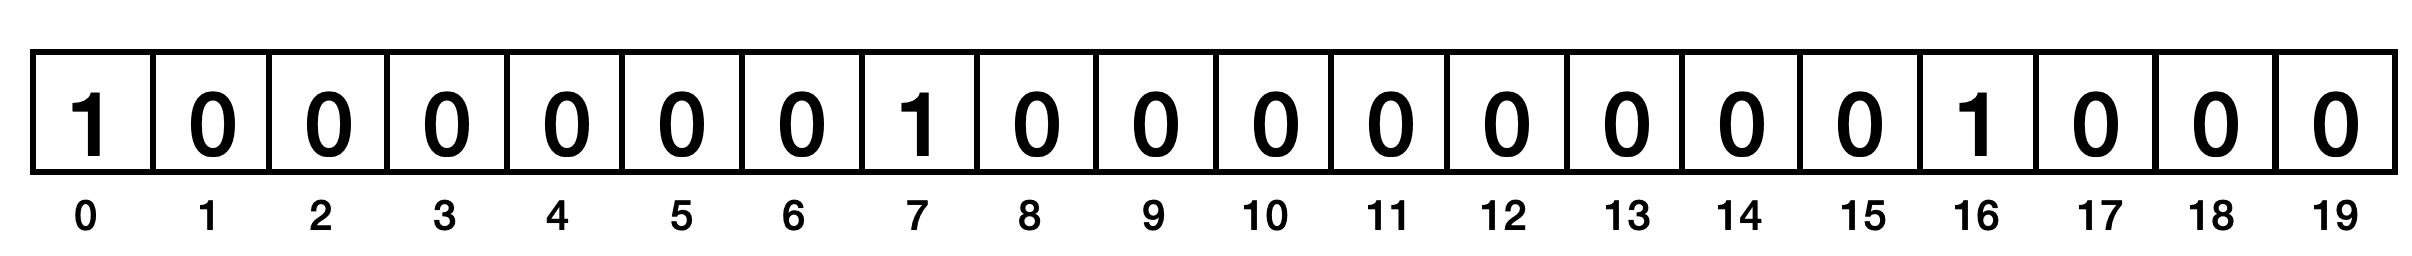
\includegraphics[width=1.0\textwidth]{images/cromosoma.png}
  \caption{Ejemplo de representacion de estado con un vector booleano}
  \label{fig:cromosoma}
\end{figure}

En este caso, las posiciones 0, 7 y 16 del vector están establecidas como verdaderas (según el orden asignado a los métodos de la API), mientras que las demás posiciones están establecidas como falsas. Esta configuración representa el subconjuto de métodos:
\vspace{5pt} 

\begin{lstlisting}[numbers=none, caption=Métodos generadores de objetos que representa el cromosoma de la Figura 2, captionpos=b, frame=tb , xleftmargin=0pt, basicstyle=\scriptsize]
  (0)  NodeCachingLinkedList()
  (7)  addFirst(Object)
  (16) removeFirst()
\end{lstlisting}

\section{Funciones objetivo}
\label{sec:fitness}
% 2- función de valoración
% también denominada función de aptitud en algoritmos genéticos

Una función objetivo, también conocida como función de costo o función de valoracion, es una función matemática que mide la calidad de una solución candidata dentro del espacio de búsqueda \cite{Russell:2009}. Esta función asigna un valor numérico a cada estado, indicando qué tan buena o deseable es el candidato con respecto al objetivo del problema.

El propósito de la función objetivo es guiar el proceso de búsqueda hacia la mejor solución posible. Dependiendo del problema, se busca maximizar o minimizar el valor de la función. En problemas de maximización, se priorizan los estados con valores más altos, mientras que en problemas de minimización, se favorecen aquellos con valores más bajos.

La función objetivo es una parte fundamental de los algoritmos de búsqueda local. Estos algoritmos utilizan la función objetivo para evaluar y comparar diferentes estados candidatos a medida que exploran el espacio de búsqueda en busca de la mejor solución posible.

En nuestros algoritmos, hemos desarrollado dos funciones objetivo distintas para guiar el proceso de búsqueda. 
Cada una de ellas con su enfoque para evaluar y comparar diferentes configuraciones de métodos generadores de objetos.

Como el conjunto de objetos que se pueden construir con la API de un módulo es potencialmente infinito, las funciones objetivo definidas a continuación usan diferentes mecanismos para acotar el espacio de búsqueda.


\subsection{Generación Exhaustiva Acotada}
\label{sec:fitnessGE}

Dado un candidato $C$ que representa un subconjunto de métodos $M$ de la API, 
nuestra función de valuación intenta calcular el número de objetos que se pueden construir utilizando combinaciones de métodos en $M$. 
Los candidatos con valores de aptitud más altos se estima que construyen más objetos que aquellos que tienen valores de aptitud más pequeños.

Así, la primera función objetivo propuesta evalúa la capacidad de generación de objetos de un candidato $C$ realizando una generación exhaustiva acotada \cite{Politano20} usando los métodos en $M$. La función objetivo asigna un puntaje a $C$ basándose en la cantidad de objetos únicos producidos durante la generación exhaustiva acotada. Esto refleja la diversidad de objetos que se pueden generar utilizando los métodos dados. Los subconjuntos de métodos que generan más objetos serán los candidatos preferidos para ser elegidos por nuestro algoritmo como generadores de objetos.
Nuestro enfoque utiliza un generador exhaustivo acotado eficiente basado en métodos de la API \cite{Politano20}. Este generador se denomina BEAPI y es una de las contribuciones principales de este trabajo (ver Capítulo \ref{cap:beapi}).
Dado un conjunto de métodos $M$ en un candidato $C$, BEAPI explora todas las secuencias de métodos acotadas que se pueden construir usando métodos de $M$. La cota consiste de un número máximo $m$ de métodos dado por el usuario, y de un conjunto de valores primitivos empleados para instanciar los parámetros de tipo primitivo en los métodos en $M$ (e.g., enteros de \( 0 \) a \( k-1 \)).
BEAPI utiliza cada uno de estos valores para instanciar cada parámetro del tipo correspondiente. 
BEAPI cuenta la cantidad de objetos distintos creados por la ejecución de cada una de las secuencias exploradas. 
Así, para $M$ (y cotas $m$ y $k$) la función de valuación retorna el número de objetos generados por BEAPI usando $M$.

Como la cantidad de secuencias a explorar crece exponencialmente respecto de las cotas, BEAPI implementa distintas técnicas que le permiten podar significativamente el espacio de búsqueda y mejorar la eficiencia de la generación (usar el feedback de la ejecución para descartar secuencias inválidas, coincidencia de estado para evitar volver a generar repetidamente los mismos objetos, descartar secuencias que generen objetos de tamaño mayor al permitido por las cotas). Para obtener más información sobre las mismas y sobre BEAPI invitamos al lector a consultar el Capítulo \ref{cap:beapi}.

Nuestra técnica se basa en una variante de la \emph{hipótesis de la cota pequeña}, ampliamente reconocida en el testing de software \cite{Andoni:2003,jackson2006, Abad13}. La hipótesis de la cota pequeña indica que la mayoría de las fallas pueden revelarse ejercitando el software bajo test con entradas de tamaño relativamente pequeño. Nuestra hipótesis es que si dos conjuntos de métodos $M_1$ y $M_2$ generan los mismos objetos acotados (para una cota relativamente pequeña), entonces es altamente probable $M_1$ y $M_2$ sirvan para generar los mismos objetos en un contexto no acotado. Esto fue validado empíricamente en todos nuestros casos de estudio.

%\cacho{Ver con Pablo luego. Pensar en ejecucion simbolica. String es mas dificil que generar un Int, ver tabla de pesos}

\begin{lstlisting}[label=fig:rankParameters,caption=Ranking con los tipos de parametros, captionpos=b,frame=tb, float=t]
Boolean=1
Integer,Char=2
Float,Double,String=4
Object=6
\end{lstlisting}
\pp{Cambié los pesos. Quizás hay que cambiar algún cálculo en base a estos
    nuevos pesos (eran 1,2,3 y 4, pasaron a ser 1,2,4 y 6.}

Como ya se discutió en esta Sección, buscamos un conjunto minimal de generadores de objetos, donde los métodos tengan parámetros tan simples como sea posible. Por lo tanto, la cantidad de objetos generados usando BEAPI es sólo un componente de la función objetivo. Dado un conjunto de métodos $M$, representado por un candidato $C$, la función objetivo $f$ devuelve un valor real conformado por tres componentes:

\[
f(M) = \langle O(M), R(M), C(M) \rangle
\]
Donde:

\begin{itemize}
    \item $O(M)$ (Objetos): Es el número de objetos generados por el conjunto de métodos $M$ usando generación exhaustiva acotada, para un scope fijo. Este componente es el más importante, ya que los siguientes componentes sólo se usan para decidir en caso de empate respecto de $O(M)$. Recordemos que los generadores de objetos a identificar deben ser siempre suficientes, por lo que la función objetivo siempre prioriza los métodos que generen un mayor número de objetos.
    \item $R(M)$ (Redundancia): Representa la diferencia entre el número total de métodos de la API ($M_t$) y la cantidad de métodos en $M$. Esto se utiliza para desempatar entre conjuntos de métodos que generan la misma cantidad de objetos, dando preferencia a aquellos conjuntos que contengan menos métodos. En otras palabras, este componente de la función busca identificar generadores de objetos minimales.
    \item $P(M)$ (Parámetros): Es una medida ponderada de la complejidad de los
        parámetros de los métodos en $M$. \pp{Sea $m_l$ un método con parámetros $p_1: T_1,
            p2: T_2, \ldots, p_k: T_j$, la función $W(m_l)$ define el peso de los
            parámetros de $m_l$ de acuerdo al tipo de los mismos. $W$ se
            define como: $W(m_l) = \sum_{i=1}^j = T(T_i)$, donde $T$ es la función
            definida en la Tabla \ref{fig:rankParameters}, que asigna a cada
            tipo un valor predefinido. $T$ es una función definida de manera heurística, 
            que asigna un mayor peso a tipos más complejos. $T$ se definió 
            considerando pesos para los tipos que dieron buenos resultados en
            nuestra evaluación experimental, y podría reemplazarse de manera
            directa por mejores heurísticas en el futuro. Extendemos la
            definición de $W$ para conjuntos de métodos de la siguiente manera.
            Sea $M'$ un subconjunto de métodos, $W(M') = \sum_{m \in M'} W(m)$.
            Si $API$ es el conjunto total de métodos, $W(API)$ representa
            el peso máximo que podría tener un subconjunto (el conjunto que
            incluye todos los métodos). 
            Ahora estamos listos para definir $P$. Como buscamos maximizar $P$, 
            primero computaremos $W(API)$ y le restaremos el valor de $W(M)$. 
            Esto es, $P(M) = W(API) - W(M)$. Esta componente de $f(M)$ se
            utiliza para desempatar entre conjuntos de métodos que generan la
            misma cantidad de objetos y tienen la misma cantidad de métodos,
            favoreciendo subconjuntos con una menor complejidad en sus
        parámetros.}


\end{itemize}


A partir de esto, podemos definir un orden sobre esta función $f$, sean dos
métodos $M_1$ y $M_2$ tales que: 

\( f(M_1) = \langle O(M_1), R(M_1), P(M_1) \rangle \) y

\( f(M_2) = \langle O(M_2), R(M_2), P(M_2) \rangle \) 
\vspace{5pt} 

el orden se define de la siguiente forma:

\[
f(M_1) > f(M_2) \quad \text{si y solo si:}
\]

\begin{enumerate}
    \item \( O(M_1) > O(M_2) \), o
    \item \( O(M_1) = O(M_2) \) y \( R(M_1) > R(M_2) \), o
    \item \( O(M_1) = O(M_2) \), \( R(M_1) = R(M_2) \), y \( P(M_1) > P(M_2) \).
\end{enumerate}

En otras palabras, se compara primero el número de objetos \( O(M_1) \) con \( O(M_2) \). 
Si son iguales, se compara la redundancia \( R(M_1) \) con \( R(M_2) \), y si ambos son iguales, 
se compara la complejidad de los parámetros \( P(M_1) \) con \( P(M_2) \).

Para ilustrar este concepto, consideremos los siguientes ejemplos.

En el primer caso, tenemos dos conjuntos de métodos:
\vspace{5pt} 

\begin{lstlisting}[numbers=none, caption=Conjunto de métodos \( M_1 \)]
  NodeCachingLinkedList()
  addFirst(Object)
  removeFirst()
\end{lstlisting} 


\begin{lstlisting}[numbers=none, caption=Conjunto de métodos \( M_2 \)]
  NodeCachingLinkedList()
  addFirst(Object)
\end{lstlisting}


Obtenemos las siguientes triplas:

\[
f(M_1) = \langle 15, 17, 4 \rangle \quad \text{y} \quad f(M_2) = \langle 12, 18, 4 \rangle
\]
\pp{4 no puede ser para el tercer componente. Porque está definido como la suma
de la API - el peso de los métodos. Debería dar un número bastante grande.}
\pp{Por qué el segundo componente da esos valores? Explicarlo.}

Dado que el conjunto \( M_1 \) genera más objetos (15 frente a 12) \pp{15? Es
demasiado chico, cuál es el scope de esto?}, \( f(M_1) > f(M_2) \). Esto implica que \( M_1 \) es capaz de generar más instancias, mientras que \( M_2 \) no puede generar algunas que requieren métodos para agregar nodos a la lista cache.

En el segundo caso, ambos conjuntos generan la misma cantidad de objetos (15), pero \( M_4 \) tiene un método adicional:
\vspace{10pt} 

\begin{lstlisting}[numbers=none,label=fig:NCLbuilders3, caption=Conjunto de métodos \( M_3 \)]
  NodeCachingLinkedList()
  addFirst(Object)
  removeFirst()
\end{lstlisting}

\vspace{10pt} 

\begin{lstlisting}[numbers=none,label=fig:NCLbuilders4, caption=Conjunto de métodos \( M_4 \)]
  NodeCachingLinkedList()
  addFirst(Object)
  add(Object)
  removeFirst()
\end{lstlisting}


Las triplas resultantes son:

\[
f(M_3) = \langle 15, 17, 4 \rangle \quad \text{y} \quad f(M_4) = \langle 15, 16, 4 \rangle
\]
\pp{4 no puede ser para el tercer componente. Porque está definido como la suma
de la API - el peso de los métodos. Debería dar un número bastante grande.}
\pp{Por qué el segundo componente da esos valores? Explicarlo.}

Aunque ambos conjuntos generan la misma cantidad de objetos, \( M_3 \) tiene una redundancia menor (16 frente a 17). Esto significa que \( f(M_3) > f(M_4) \), ya que \( M_3 \) contiene menos métodos redundantes.

En el tercer caso, los conjuntos tienen la misma cantidad de objetos y métodos, pero \( M_6 \) tiene más parámetros en el método \( add(int, Object) \):
\vspace{10pt} 

\begin{lstlisting}[numbers=none,label=fig:NCLbuilders5, caption=Conjunto de métodos \( M_5 \)]
  NodeCachingLinkedList()
  addFirst(Object)
  removeFirst()
\end{lstlisting}

\vspace{10pt} 

\begin{lstlisting}[numbers=none,label=fig:NCLbuilders6, caption=Conjunto de métodos \( M_6 \)]
  NodeCachingLinkedList()
  add(int, Object)
  removeFirst()
\end{lstlisting}

\vspace{10pt} 

Obtenemos las siguientes triplas:

\[
f(M_5) = \langle 15, 17, 4 \rangle \quad \text{y} \quad f(M_6) = \langle 15, 17, 6 \rangle
\]
\pp{4 no puede ser para el tercer componente. Porque está definido como la suma
de la API - el peso de los métodos. Debería dar un número bastante grande.}
\pp{Por qué el segundo componente da esos valores? Explicarlo.}

Ambos conjuntos generan la misma cantidad de objetos y tienen la misma
redundancia, pero \( M_6 \) tiene mas parámetros \pp{No importa el número de
    parámetros sino su complejidad. Hay que calcular bien el tercer componente
para este caso}. (el método \( add(int, Object)
\) tiene un parámetro adicional). Como resultado, \( f(M_6) > f(M_5) \), debido
a que preferimos una menor complejidad en los parámetros. 

\cacho{Poner el total de parametros que tiene NCL, buscar en experimentos}\pp{O
calcularlo a mano, no es difícil.}


%Para este propósito, desarrollamos la herramienta BEAPI, que se discute con más detalle en el Capítulo \ref{cap:beapi}. En resumen, primero exploramos exhaustivamente todas las posibles combinaciones de secuencias de los métodos de $M$. Luego, utilizamos un conjunto fijo de valores primitivos (enteros del 0 a $k-1$) con los cuales probar nuestros métodos cuando requieren valores primitivos.

%En segundo lugar, descartamos las secuencias de métodos que crean objetos con más de $k$ objetos (de cualquier tipo) para evitar construir objetos más grandes de lo necesario. Para lograr esto, canonizamos los objetos generados por la ejecución de cada secuencia y descartamos la secuencia si algún objeto tiene un índice igual o mayor que $k$.

%En tercer lugar, ampliamos esta generación con coincidencia de estado. Esto se debe a que, en la generación de pruebas, a menudo hay muchas secuencias de pruebas que producen el mismo objeto. Por ejemplo, insertar en una colección y luego eliminar el mismo elemento resulta en muchos casos en exactamente la misma estructura antes de la inserción. Nuestro enfoque asume que las ejecuciones de rutinas son deterministas con respecto a sus entradas. Bajo esta suposición, se deduce que, para generar un conjunto exhaustivo acotado de estructuras, solo necesitamos guardar una secuencia de prueba para crear cada estructura diferente en el conjunto, y que todas las siguientes secuencias de prueba que generen la misma estructura se pueden descartar.


\subsection{Cobertura de código}
\label{sec:fitnessRandoop}

\pp{Como la generación exhuastiva acotada puede ser costosa computacionalmente,
    proponemos aquí una heurística para computar la función objetivo que debería
    dar lugar a una mejor eficiencia en los algoritmos de cómputo de métodos
generadores.} Así, la segunda función objetivo se basa en generar test suites
de manera automática (aleatoria) utilizando un suconjunto candidato de métodos,  
y medir la cobertura de código que alcanzan estas test suites. 
La cobertura se mide en términos de las líneas de código y las ramas del
programa que son ejercitadas por los tests \pp{hacer referencia a la sección
correspondiente de background y mirar que matcheen los términos usados}.
Esta métrica nos da una idea de qué tan bien los tests generados usando el
subconjunto de métodos pueden cubrir las diferentes partes del programa, 
lo que nos permite evaluar un aspecto importante de la calidad de las test
suites generadas por los métodos.
% PABLO: Esto está en background
%Los criterios de evaluación incluyen:
%\begin{itemize}
%    \item \textbf{Cobertura de líneas de código:} Porcentaje de líneas de código ejecutadas al correr los test suites.
%    \item \textbf{Cobertura de ramas:} Porcentaje de decisiones (\textit{branches}) exploradas en el flujo de ejecución del programa.
%\end{itemize}
Por ejemplo, si se genera una test suite que cubre 100 líneas de código y 20 ramas de la API, 
la función objetivo combina estas métricas en un puntaje compuesto.

Para ello, se calcula la proporción de líneas y ramas cubiertas respecto del total disponible, 
y se ponderan según su importancia relativa. Así, la cobertura alcanzada por una
test suite puede definirse como:

\[
\text{Cob}(M) = \alpha \cdot \frac{L_M}{L_{\text{total}}} + \beta \cdot \frac{B_M}{B_{\text{total}}}
\]

donde $\alpha$ es $0.4$ y $\beta$ es $0.6$ para darle un peso mas importante a la cobertura de ramas.
Este enfoque es especialmente útil en casos donde el objetivo es favorecer
métodos que sean útiles para generar tests que ejerciten la mayor cantidad
posible de ramas del código.
En el contexto de nuestra tesis, hemos realizado modificaciones en la
herramienta \emph{Randoop} (descrita en la sección
\ref{sec:feedback-directed-test-gen})
de manera que las test suites generadas sean de utilidad para averiguar si un conjunto de 
métodos dados es un buen conjunto de métodos generadores.

La heurística para averiguar si un
subconjunto de métodos $M$ es un buen conjunto de generadores se basa en
realizar una primera ejecución de Randoop utilizando sólo los métodos en $M$ para
generar un conjunto de secuencias de test que generen objetos $tests_{obj}$. En
otras palabras, se asume que los métodos en $M$ son generadores de objetos (y
en la segunda etapa se busca evaluar si efectivamente lo son).
Luego, estas secuencias se extienden en una ejecución de Randoop subsiguiente,
pero esta vez usando los métodos restantes de la API. El objetivo de esta
segunda ejecución es maximizar la cobertura de código obtenida por la suite. 
De esta manera, si los métodos en $M$ son un buen conjunto de generadores de objetos
la cobertura obtenida por la suite final será alta; en caso contrario será baja. 
Por ejemplo, si la primera ejecución no puede construir muchos objetos, extender 
$tests_{obj}$ no dará lugar a buena cobertura.

El algoritmo de Randoop modificado para la detección de métodos generadores se muestra 
en la Figura \ref{alg:fitnessRandoop}.
Primero, se realiza una ejecución de Randoop sólo con los métodos de $M$ para
generar secuencias de test, $tests_{obj}$ (línea 6), que usan estos métodos para construir objetos \pp{Tiene state
matching activado esto?}. Esta ejecución utiliza un 40\% del tiempo total
asignado, \texttt{S} (ver $S_1$ en la línea 2). 
La función \texttt{GenerarNuevasSecuencias} (líneas 9-35) es la encargada de
producir estas secuencias de test. Esta función realiza su tarea utilizando 
la estrategia de generación aleatoria descrita en la Sección~\ref{sec:feedback-directed-test-gen}, basada en el enfoque de Randoop. 

\pp{Meter el algoritmo en un float para que encaje bien? el vspace no funciona}

\begin{algorithm}[htbp]
    \SetAlgoLined
    \KwIn{Métodos de la API $API$, subconjunto de métodos $M \subseteq API$,
    tiempo total $S$}
    \KwOut{Conjunto final de tests generados}
    
    \SetKwFunction{FMain}{GenerarTests}
    \SetKwFunction{FGen}{GenerarNuevasSecuencias}
    \SetKwProg{Fn}{Function}{:}{}
    \BlankLine


    \Fn{\FMain{$API$, $M$, $S$}}{
    
        $S_1 \leftarrow 0.4 \cdot S$\;
        $S_2 \leftarrow 0.6 \cdot S$\;
    
        $M_{gen} \leftarrow$ $M$\;
        $M_{nogen} \leftarrow$ $API - M$\;
    
        $tests_{obj}, tests_1 \leftarrow$ \FGen{$M_{gen}$, $S_1$}\;
        $prev_2, tests_2 \leftarrow$ \FGen{$M_{nogen}$, $S_2$, $tests_{obj}$}\;
    
        \Return{$tests_2$}\;
    }
    
    \BlankLine

    \Fn{\FGen{$M'$, $S'$, $T_0$}}{

    $tests \leftarrow \emptyset$\;
    $prev \leftarrow T_0$\;

    \While{tiempo transcurrido $< S'$}{
        Seleccionar aleatoriamente $m(p_1:T_1, \ldots, p_m:T_m) \in M'$\;
        \For{$p_i:T_i$ de $m$}{
            \If{$T_i$ es primitivo}{
                $S_i \leftarrow$ valor primitivo para $T_i$ tomado
                aleatoriamente de las semillas\;
            }\Else{
                $S_i \leftarrow$ secuencia aleatoria $\in prev$ que crea objeto de tipo $T_i$\;
            }
        }
        $test \leftarrow S_1; \ldots; S_m; m(v_1,\ldots,v_m)$\;
        $res \leftarrow ejecutar($test$)$\;
        \If{res = falla} {
            \Return{$\{ test \}$}\;
        }   
        \If{res = inválido} {
            // No se guarda test para futuras extensiones
        }       
        \If{res = exito} {
            $prev \leftarrow prev \cup \{test\}$\;
        }        
        $tests \leftarrow tests \cup \{test\}$\;
    }
    \Return{$tests$}\;
    }
    
    \caption{GenerarTests}
    \label{alg:fitnessRandoop}
    \end{algorithm}
    

\pp{Hace falta el número máximo de tests W en el algoritmo o lo podemos sacar? Me suena raro
pero podría estar comiéndome algún caso.} \cacho{Hecho, no hace falta}

Más adelante, se realiza una segunda ejecución
de Randoop usando las secuencias de test $tests_{obj}$ como punto de partida para
generar otras secuencias nuevas, utilizando los restantes métodos de la API
($API - M$; ver línea 5). El resultado de esta ejecución es la suite de tests final
$tests_2$ (línea 7), retornada por el algoritmo (línea 8).
La segunda ejecución usa un 60\% del tiempo
asignado \texttt{S} (ver $S_2$ en la línea 3). 
Nuevamente, la producción de secuencias de test se hace invocando a
\texttt{GenerarNuevasSecuencias}.

\pp{Muchos errores de ortografía había en esta y en otras secciones! Instalar un spell
checker para latex.}

Usamos el algoritmo \ref{alg:fitnessRandoop} para computar $Cob$ de la siguiente manera.
Primero, se genera una test suite para un conjuto de métodos dado $M$, con un tiempo límite
de generación $S$ fijo (determinado experimentalmente). Luego, se mide  
 la cobertura de líneas y de ramas obtenida por la test suite, y se computa
 $Cob$ aplicando la fórmula \ref{} \pp{poner fórmula} con estos valores.

La función objetivo que utilizamos para evaluar la calidad de un candidato, 
representado por un conjunto de métodos $M$, se define como una tripla al igual 
que la función de la sección \ref{} \pp{Ref.}:

\[
f(M) = \langle Cob(M), R(M), C(M) \rangle
\]
\pp{Cambiar $f$ por $f'$, sino parece que fuera la misma función}

Donde:

\begin{itemize}
    \item $Cob(M)$ (Cobertura): Es el número de ramas y lineas cubiertas
        (\pp{ref a la fórmula de Cob}) por la
        suite generada por el algoritmo \ref{} \pp{Ref.}, utilizando $M$ como
        entrada. 
    Este componente tiene la mayor importancia, ya que refleja directamente la
    efectividad de los tests al cubrir líneas y ramas de la API.
\item $R(M)$ (Redundancia): Diferencia entre el número total de métodos de la
    API ($M_t$) y la cantidad de métodos en $M$. Se define igual que para la
    función objetivo basada en generación exhuastiva acotada de la sección \ref{} \pp{Ref.}.
    \item $P(M)$ (Parámetros): Medida ponderada de la complejidad de los
        parámetros de los métodos en $M$. También mantuvimos el mismo cálculo
        que para la función objetivo basada en generación exhaustiva acotada.
\end{itemize}

Volvamos al ejemplo que usamos durante este capítulo. En el primer caso tenemos los siguientes métodos:
\vspace{5pt} 

\begin{lstlisting}[numbers=none, caption=Conjunto de métodos \( M_1 \)]
  NodeCachingLinkedList()
  addFirst(Object)
  removeFirst()
\end{lstlisting} 

y en el segundo caso tenemos:

\begin{lstlisting}[numbers=none, caption=Conjunto de métodos \( M_2 \)]
  NodeCachingLinkedList()
  addFirst(Object)
\end{lstlisting}


Para estos casos, se ejecuta el algoritmo \ref{} \pp{Ref.} y se obtienen test suites.
A partir de estas, se ejecutan y se analiza la cobertura que se obtiene, cuyo
resultado se muestra a continuación:

\[
f(M_1) = \langle 15, 17, 4 \rangle \quad \text{y} \quad f(M_2) = \langle 12, 18, 4 \rangle
\]

\pp{El ejemplo está incompleto. 15 no sé qué es, habría que decir más o menos
    que cobertura obtuvo, por qué un conjunto de métodos obtiene más cobertura
    que el otro, etc.. Sino así como está no aclara mucho. Hay que arreglar todo lo que había que arreglar en la sección previa también (ej. valuaciones para los parámetros.}

En nuestra evaluación experimental, ambas funciones objetivo son utilizadas como
parte de los algoritmos de búsqueda implementados, para analizar sus ventajas y
desventajas en la práctica. 

\section{Algoritmos para la Identificación de Métodos Generadores de Objetos}
\label{sec:algorithms}

\pp{En algún lugar habría que meter un gráfico de cómo funciona la técnica a alto nivel. Creo que en alguna de las slides teníamos algo así.} 
\cacho{Poner algo de dibujitos algo sobre el flujo de la tecnicas. Pedir a Vale el de BEAPI y adaptarlo aca, asi quedan del mismo formato}

\subsection{Algoritmo Genético}
\label{alg:approachGA}

Los algoritmos genéticos \cite{Goldberg:1989} son algoritmos de búsqueda guiada no exhaustivos, 
basados en una estrategia de ascenso de colinas \cite{Russell:2009}. El espacio de búsqueda está 
compuesto por un conjunto generalmente muy grande de individuos (los candidatos), y
el objetivo de la búsqueda es encontrar un individuo con las características deseadas. 
A diferencia de los algoritmos de búsqueda clásicos, los algoritmos genéticos mantienen un conjunto de individuos,
llamado la población, y la búsqueda progresa seleccionando iterativamente un número de individuos de la población, 
utilizando estos para la evolución (construyendo nuevos individuos a partir de estos), 
y dejando fuera algunos individuos del conjunto total (los ``viejos'' y los ``nuevos'').
La selección de individuos para la evolución de la población, así como la eliminación de individuos, 
son guiadas por una función de aptitud, la función heurística utilizada para guiar la búsqueda. 
Esta función se aplica a los individuos, y su resultado es generalizable también a la población 
(por ejemplo, la aptitud de la población puede tomarse como la aptitud de su individuo ``más apto'').
Esta función captura las características deseadas en la búsqueda, y por lo tanto puede usarse como un 
criterio de detención (por ejemplo, el algoritmo se detiene después de encontrar un individuo con una 
aptitud superior a un umbral determinado). Finalmente, los individuos suelen llamarse cromosomas y 
se representan como vectores de genes que capturan sus características. Esta idea está estrechamente relacionada 
con la forma en que se construyen los nuevos individuos: al representar a los candidatos como vectores de 
características independientes, se pueden construir nuevos candidatos combinando parte de las características 
de un individuo con parte de las características de otro, o cambiando arbitrariamente una característica de 
un individuo dado. Estas dos formas de evolución se llaman cruzamiento y mutación, respectivamente, y son el 
mecanismo tradicional para construir nuevos candidatos a partir de los existentes en los algoritmos genéticos. 
%Para más detalles, remito al lector a \cite{Michalewicz:1996}.

A continuacion explicaremos en detalle los distintos componentes del algoritmo genético que hemos implementado.

\subsubsection{Población}

En el contexto de un algoritmo genético, la población se refiere a un conjunto de individuos o soluciones candidatas \cite{Goldberg:1989}. 
Cada individuo de la población representa una posible solución al problema que se está tratando de resolver.

Para nuestro algoritmo, los individuos se representan como vectores de bits, como se describió en la Sección \ref{sec:estados}. 
La población inicial puede generarse de manera aleatoria o definirse según un criterio específico para mejorar la exploración del espacio de búsqueda. 
En nuestro caso, optamos por una población inicial estructurada, donde cada individuo representa un estado \emph{singleton}, es decir, 
un vector de bits en el que solo un único método está activado. Esta estrategia permite una mejor exploración inicial del espacio de soluciones, 
facilitando la combinación progresiva de métodos a lo largo de las generaciones.

En un algoritmo genético, la población evoluciona a lo largo de las generaciones a través de operaciones de selección, 
cruzamiento (\emph{crossover}) y mutación \cite{Goldberg:1989}

En cada iteración del algoritmo, los individuos más aptos tienen más probabilidad de ser seleccionados para cruzarse y/o mutarse, 
y así crear nuevos individuos que a su vez formarán parte de la población de la siguiente generación. Con el tiempo, se espera que la población evolucione y
mejore su aptitud en función del criterio de optimización establecido por la función objetivo.

En nuestro caso, la población está limitada a un tamaño de 50 individuos a lo largo del proceso evolutivo. Como es típico en los algoritmos genéticos, 
el tamaño de la población fue determinado empíricamente, probando distintos valores y eligiendo aquel que mejor rendimiento obtuvo en nuestros experimentos.

En nuestro algoritmo, tenemos una población inicial de 50 individuos. Durante todo el proceso evolutivo, la población está limitada a un tamaño de 100 individuos. Cómo es típico para los hiperparámetros de los algoritmos genéticos determinamos el tamaño de la población empíricamente, probando distintos valores y utilizando el que mejor funcionaba en nuestros experimentos. 
%El método de prueba y error es comúnmente utilizado en computación evolutiva para definir los parámetros de búsqueda de manera adecuada. Es importante mencionar que si bien elegimos estos valores basándonos en los resultados de experimentos en un solo caso de estudio, luego utilizamos los mismos valores para el resto de los casos de estudio.

A medida que el algoritmo avanza, se aplican operadores genéticos como el cruzamiento y la mutación para crear nuevos individuos a partir de la población actual.

\subsubsection{Selección}

La selección en los algoritmos genéticos es el proceso de elegir qué individuos de la población actual participarán en la reproducción y darán lugar a la siguiente generación \cite{Goldberg:1989}. En este proceso, se otorgan mayores probabilidades de selección a los individuos más aptos, es decir, aquellos que tienen un mejor valor de la función objetivo \cite{Goldberg:1989}
La idea detrás de la selección es favorecer la transmisión de características deseables de los individuos más aptos a las generaciones futuras, para así mejorar gradualmente la calidad de las soluciones.

En nuestro enfoque, hemos utilizado un operador de selección tipo torneo (\emph{tournament}) \cite{Goldberg:1989}. Este enfoque funciona de la siguiente manera: se selecciona aleatoriamente un grupo de $t$ individuos de la población y se los pone a ``competir'' entre sí. El individuo más apto (con valor de la función objetivo) dentro de este grupo es seleccionado para participar en la reproducción. El tamaño del torneo $t$ (la cantidad de individuos que compiten entre sí) es un hiperparámetro del algoritmo. En nuestro caso, utilizamos un tamaño de torneo de 4, seleccionado empíricamente.

El operador de selección tipo torneo ofrece una forma eficiente de elegir individuos y típicamente da lugar una buena diversidad de individuos en la población \cite{Goldberg:1989}. Es eficiente porque los torneos pueden paralelizarse, debido a que son independientes entre si. Además, es un operador muy flexible, ya que permite adaptar la velocidad de convergencia del algoritmo variando $t$. Valores más grandes de $t$ producen una mayor probabilidad de selección de los invidividuos más aptos, lo que acelera la convergencia, y viceversa. 

Nuevamente, elegimos este operador de selección porque dió los mejores resultados en nuestros experimentos (también probamos otros operadores típicos como selección por ruleta, selección por ranking \cite{Goldberg:1989}.

\subsubsection{Operadores Genéticos: Cruzamiento}
El cruzamiento, también conocido como \emph{crossover}, es uno de los operadores fundamentales en los algoritmos genéticos. 
Este proceso permite combinar la información genética de dos individuos seleccionados de la población (denominados padres) para generar nuevos individuos (descendientes o hijos), 
quienes heredan características de ambos progenitores.
De este modo, el algoritmo explora nuevas combinaciones genéticas y mejora la diversidad de la población.  

En nuestro enfoque, empleamos el operador de cruzamiento de dos puntos \cite{goldberg1989genetic}, ya que obtuvo los mejores resultados en nuestros experimentos.  
La Figura \ref{fig:crossover} ilustra este procedimiento aplicado a dos individuos representados como vectores de bits.  
En este ejemplo, los puntos de cruzamiento seleccionados son el tercer y el sexto bit.  
El primer descendiente hereda los primeros tres bits del primer padre, los siguientes tres bits del segundo padre y los bits restantes nuevamente del primer padre.  
De manera análoga, el segundo descendiente toma los primeros tres bits del segundo padre, intercambia los siguientes tres con el primer padre y conserva los últimos cuatro bits del segundo padre.  
En nuestro contexto de detección de métodos generadores de objetos, cada posición en el vector representa la presencia ('1') o la ausencia ('0') de un método de la API.  
Por ejemplo, la posición 0 puede corresponder a un constructor de listas, la
posición 1 a un método de inserción, etc.  
Al aplicar el operador de cruzamiento, los hijos heredan distintas subsecuencias de métodos
de los padres. Este mecanismo favorece la exploración del espacio de búsqueda y permite descubrir configuraciones más diversas y potencialmente óptimas. 

\begin{figure}
  \centering
  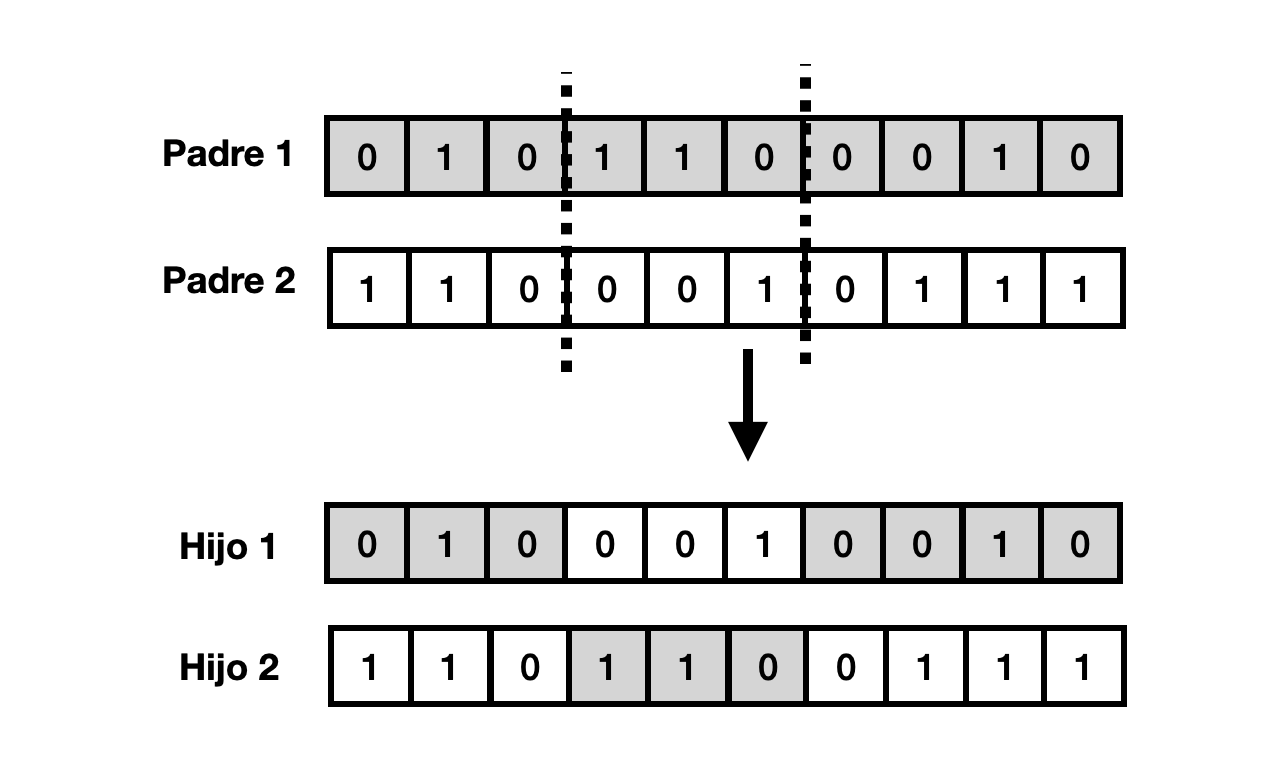
\includegraphics[width=0.9\textwidth]{images/crossOver.png}
  \caption{Ejemplo de crossover de dos puntos con dos cromosomas.}
  \label{fig:crossover}
\end{figure}


En nuestro algoritmo, utilizamos una tasa de cruzamiento de 0.30 (\emph{crossover rate}), lo cual significa que en cada generación aproximadamente el 30 por ciento de los individuos serán seleccionados para cruzarse y crear nuevos descendientes. Este valor fue obtenido a partir de evaluaciones experimentales que hemos realizado para nuestros casos de estudio.

\subsubsection{Operadores Genéticos: Mutación}

La mutación es un operador fundamental en los algoritmos genéticos, encargado de introducir cambios aleatorios en los cromosomas para aumentar la diversidad en la población.  
Cada bit del cromosoma tiene una pequeña probabilidad de ser modificado, lo que en una representación binaria implica invertir su valor ('0' a '1' o viceversa).  
Este mecanismo, denominado \emph{mutación por inversión de bits}, es especialmente adecuado para representaciones binarias como la utilizada en nuestro enfoque. 

La Figura \ref{fig:mutation} muestra un ejemplo de mutación en el que las posiciones 1, 4, 5 y 7 del cromosoma fueron seleccionadas para ser alteradas.  
Aunque la mutación es un proceso aleatorio, su probabilidad se mantiene baja para evitar cambios drásticos que puedan comprometer la convergencia del algoritmo.  
En nuestro caso, utilizamos una probabilidad de mutación de 0.08, es decir, cada bit de un individuo tiene un 5\% de probabilidad de cambiar de estado.  
Este valor fue determinado experimentalmente para equilibrar la exploración y la preservación de soluciones prometedoras.

Para nuestro caso concreto, como ya explicamos, cada posición del cromosoma representa un método específico de la API, entonces una mutación en la posición 2 implicaría activar o desactivar el método
correspondiente en el individuo.
Este tipo de variaciones permite explorar diferentes combinaciones de subconjuntos de métodos que de otra manera no se generarían.  

\begin{figure}
    \centering
    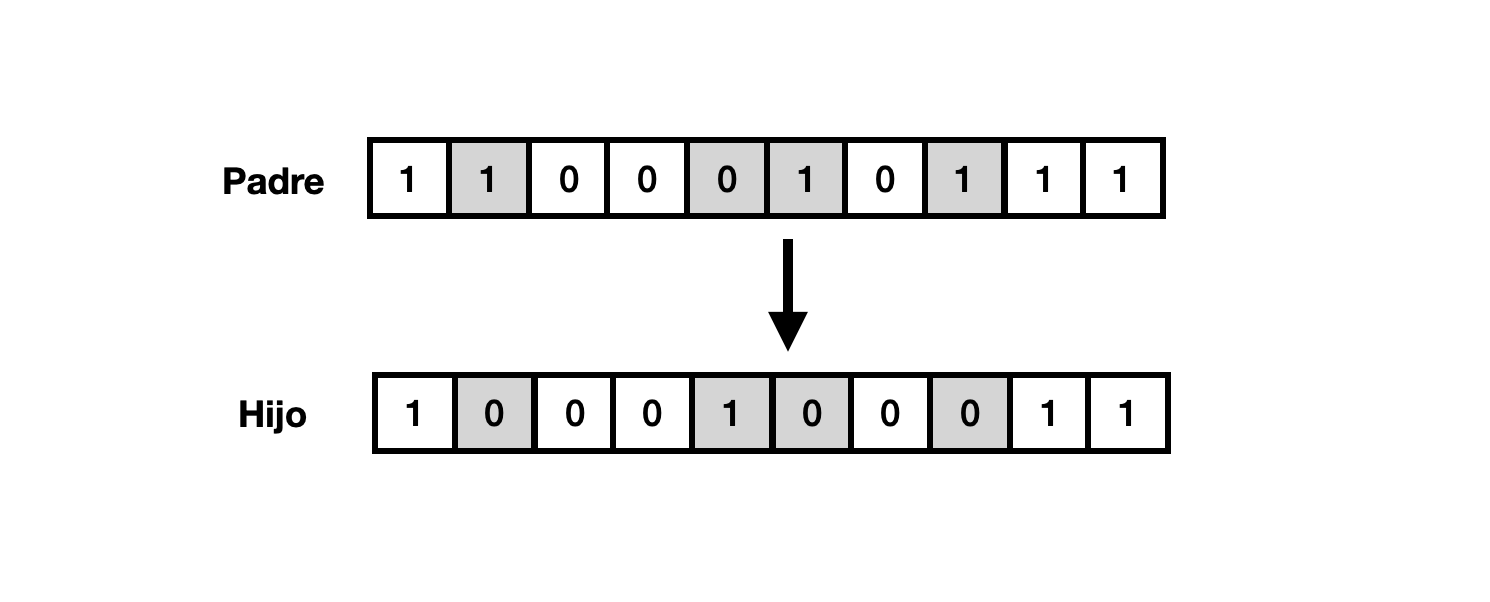
\includegraphics[width=0.9\textwidth]{images/mutation.png}
    \caption{Ejemplo de mutación por inversión de bits.}
    \label{fig:mutation}
    \end{figure}
\subsubsection{Pseudocódigo del algoritmo genético}

El algoritmo~\ref{alg:enfoqueGA} muestra un pseudocódigo del algoritmo genético que definimos para la búsqueda de métodos generadores de objetos.


\begin{algorithm}
  \caption{Algoritmo genético para la identificación de métodos generadores de
  objetos}
  \label{alg:enfoqueGA}
  \begin{algorithmic}[1]
  
  \STATE $P \gets$ generar población aleatoria
  \FOR{$i \gets 0$ \TO $numEvoluciones$}
      \STATE $P \gets$ $popSize$ cromosomas más aptos de $P$
      \FOR{$j \gets 1$ \TO $\text{tasaC} \times |P|$}
          \STATE $C_1, C_2 \gets$ dos cromosomas más aptos 
          \STATE cruzar($C_1, C_2$)
      \ENDFOR
      \FORALL{cromosomas en $P$}
          \STATE mutar $1/\text{tasaMutacion}$ genes
      \ENDFOR
  
    \STATE $C \gets$ mejor cromosoma de $P$
    \STATE $actual \gets$ estado inicial

    \IF{aptitud de $C$ es constante durante $maxIter$}
        \STATE detener algoritmo
    \ENDIF
\ENDFOR

\end{algorithmic}
\end{algorithm}


Los elementos descritos anteriormente son las partes constitutivas del algoritmo genético que implementa nuestro enfoque. 
Nótese que el algoritmo~\ref{alg:enfoqueGA} sigue la estructura típica de un algoritmo genético. 

La población inicial se genera produciendo todos los cromosomas factibles con un
único método disponible (vectores con falso en todas las posiciones excepto una,
establecida en verdadero) (línea 1) \pp{esto no coincide con el pseudocódigo}. 
Luego, comienza a evolucionar la población de forma iterativa (líneas 2-14). 
Al inicio de cada iteración, el algoritmo descarta algunos individuos para controlar el tamaño de la población, conservando los $popSize$ individuos más aptos de la población actual y eliminando el resto (línea 3).

\pp{Cuál es la función objetivo del algoritmo genético?}

Posteriormente, el algoritmo realiza un cruzamiento de dos puntos en individuos
seleccionados aleatoriamente (líneas 4-7). \pp{No. Debería usar tournament para
hacer selección. Tournament selection no aparece en ningún lado del
pseudocódigo, está incompleto o es otra cosa diferente al algoritmo real.
Tenemos que juntarnos a ver esto.}
El cruzamiento se aplica un número de veces proporcional al tamaño de la población $popSize$, 
determinado por el producto de $popSize$ y la tasa de cruzamiento $cRate$ ($0
\leq cRate \leq 1$). \pp{cRate no está en el algoritmo}. \pp{El resultado del
cruzamiento no se sabe a qué población va a parar, parece que se tirara de la
forma en que está el pseudocódigo.}
Luego, el algoritmo muta los individuos (líneas 8-10) cambiando el valor de cada
uno de sus genes con probabilidad $mRate$ ($0 \leq mRate \leq 1$) \pp{mRate no
está en el algoritmo. El resultado de mutar tampoco se sabe dónde se guarda.}. 
Todos los nuevos individuos creados por las operaciones de cruzamiento y
mutación se agregan a la población \pp{dónde en el pseudocódigo?}.

El algoritmo se detiene después de $numEvo$ \pp{No está en el algoritmo}
evoluciones, donde $numEvo$ es un parámetro del algoritmo \pp{No están
declarados los parámetros del algoritmo, habría que declararlos al inicio para
que queden más claros}. 
%Cabe destacar que no tenemos un valor objetivo para nuestra función de fitness, 
%ya que un conjunto no probado de métodos podría producir más  que las observadas hasta el momento. 
Nuevamente, existe un compromiso al elegir un buen valor para $numEvo$: un número mayor aumenta la precisión del algoritmo pero incrementa su tiempo de ejecución, 
mientras que un número menor lo hace más rápido pero podría no encontrar el
mejor conjunto de generadores de objetos.

\pp{Qué hacen las líneas 11, 12, 13-15? No están en el texto.}

Como es habitual, determinamos valores para los parámetros del algoritmo que
funcionan bien de manera experimental. Luego de realizar experimentos en
varios casos de estudios y con diferentes valores para los párametros 
elegimos $numEvo=20$, $popSize=50$, $cRate=0.35$, $mRate=0.08$ 
y $maxIter=5$. 

%Cabe destacar que, si quitamos la complejidad de la función de aptitud, nuestro algoritmo evolutivo es bastante estándar, por lo que no es sorprendente que una implementación existente funcione bien para nuestros propósitos. Por supuesto, realizar mejoras en el algoritmo evolutivo y ajustar sus parámetros (como las tasas de cruce y mutación) podría acelerar los tiempos de ejecución.

También implementamos una versión simple de nuestro enfoque que utiliza
múltiples hilos (multi-threading), lo que ayuda a mejorar el rendimiento.
Básicamente, en cada iteración se crean t copias de la población actual, donde t
es el número de hilos disponibles. Luego, cada réplica de la población
evoluciona de forma independiente. Cuando todos los hilos terminan, se conservan
los 50/t individuos más aptos de la población evolucionada por cada hilo, y
estos se utilizan para construir la población de la siguiente iteración del
algoritmo. \pp{No estoy seguro que nos convenga mantener este párrafo. Jenetics quizás
maneje los hilos solo? O los implementaste vos? Un jurado que sepa de genéticos nos puede pegar por
todos lados.}

Para implementar el algoritmo genético, utilizamos una biblioteca muy popular en Java llamada \emph{Jenetics}\footnote{https://jenetics.io/}. Esta biblioteca está diseñada específicamente para algoritmos evolutivos y nos proporcionó las herramientas necesarias para desarrollar nuestro enfoque genético.
\emph{Jenetics} es una biblioteca robusta y versátil que ofrece una amplia gama de funcionalidades para la implementación de algoritmos genéticos. Nos permitió definir y manipular genes, cromosomas y poblaciones, así como utilizar operadores genéticos como selección, cruzamiento y mutación. Además, cuenta con un sólido conjunto de herramientas de optimización y técnicas de evolución que nos permitieron adaptar el algoritmo a nuestras necesidades específicas.
Gracias a \emph{Jenetics}, pudimos implementar el algoritmo genético de manera eficiente y efectiva, lo que nos permitió explorar y encontrar subconjuntos óptimos de métodos \emph{builders} para las diferentes estructuras de datos en nuestro estudio. Además, \emph{Jenetics} es muy fácil de usar, con una documentación completa y una comunidad activa de usuarios que proporciona soporte y ayuda.
utivo y ajustes finos de sus parámetros (ej. tasas de cruzamiento/mutación) podrían optimizar los tiempos de ejecución.


%\subsection{Representación del Cromosoma}

%En el contexto de nuestro problema, las soluciones candidatas representan conjuntos de métodos de la API del módulo que se está analizando. Empleamos vectores de valores booleanos como representación del cromosoma. Sea $n$ el número de métodos en la API; los cromosomas en nuestro algoritmo serán vectores de tamaño $n$. Para cualquier vector, la posición $i$ será verdadera si y solo si el cromosoma contiene el $i$-ésimo método de la API. Por ejemplo, hay 34 métodos en la API de NCL (Tabla \ref{tab:ncl-api}), y los numeramos del 0 al 33. El conjunto suficiente de constructores en la Figura \ref{fig:NCLbuilders} está caracterizado por el vector con las posiciones 0, 7 y 25 configuradas como verdaderas, y las posiciones restantes configuradas como falsas. En este caso, el espacio de búsqueda completo consta de los $2^{34}$ cromosomas posibles.

% Idealmente, nos gustaría explorar todos los objetos factibles dentro de un límite pequeño $k$, 
% que pueden construirse utilizando los métodos del cromosoma actual, es decir, $BE(M, k)$.
% En otras palabras, necesitamos un generador exhaustivo limitado para el conjunto de métodos. 
% El límite $k$ representa el número máximo de objetos que se pueden crear para cada clase (en la Figura \ref{fig:ncl-instances}, 
% el número de nodos en los objetos NCL está limitado por $k=2$), 
% y el número máximo de valores primitivos disponibles (por ejemplo, enteros de 0 a $k-1$). 
% Para esto, desarrollamos un prototipo modificando la herramienta Randoop, 
% que se discute brevemente en la Sección \ref{sec:randoop}.
% Primero, alteramos Randoop para trabajar con un conjunto fijo de valores primitivos (enteros de 0 a $k-1$). 
% (Normalmente, Randoop guardaría valores primitivos que se devuelven por la ejecución de pruebas, y reutilizaría estos valores en futuras pruebas). En segundo lugar, hacemos que Randoop descarte secuencias de métodos que creen objetos con más de $k$ objetos (de cualquier tipo), para evitar que construya objetos más grandes de los necesarios. Para lograr esto, canonicemos los objetos generados por la ejecución de cada secuencia, y descartamos la secuencia si algún objeto tiene un índice igual o mayor que $k$. En tercer lugar, extendemos Randoop con extensiones de campos ``globales'', y cuando la ejecución de una secuencia termina, todos los valores de campo de los objetos generados por la secuencia se agregan a las extensiones de campos. Por ejemplo, si Randoop hubiera generado los objetos en la Figura \ref{fig:ncl-instances}, entonces las extensiones globales de campo tendrían los valores mostrados en la Figura \ref{fig:NCLextensions}. Nuestro objetivo es que, dado un límite $k$, cuando nuestra versión modificada de Randoop termine, las extensiones globales de campo contengan todos los valores de campo del conjunto exhaustivo limitado de estructuras con hasta $k$ nodos, $BE(M, k)$. El resultado de la función de aptitud para el cromosoma es el número de valores de campo en las extensiones globales calculadas por la herramienta.

% Nuestra justificación para usar conjuntos limitados de objetos es similar a la hipótesis de alcance pequeño para la detección de errores \cite{Andoni:2003}: si un conjunto de métodos no se puede usar para construir objetos pequeños que permitan diferenciarlo de otro conjunto de métodos, entonces es poco probable que estos dos conjuntos se puedan distinguir con objetos más grandes. Esta hipótesis se cumplió durante nuestra evaluación empírica en todos nuestros estudios de caso.

% Descubrimos que, además de verse afectada por el azar, nuestra herramienta rara vez deja de construir objetos que deberían agregar valores relevantes a las extensiones globales, cuando se emplean valores pequeños para $k$.


%vieja explicacion

% El algoritmo comienza con una población inicial de individuos, que son configuraciones del problema que estamos tratando de resolver. El metedo \emph{new Poblacion()} 
% es el encargado de devolvernos el conjunto de individuos iniciales con el que comenzara la busqueda.
% \pp{Antes se menciona que se genera aleatoriamente, no está en el algoritmo esto. Hay que hacer referencia a las secciones en las que se explica cada componente.}.
% \cacho{Aca comente arriba que inciiamos con una poblacion de singletons, se puede evitar decir esto, para no ensuciar el algoritmo genetico como tal}
% El algoritmo se ejecuta en ciclos repetitivos llamados generaciones. En cada generación, se crea una nueva población a partir de la población anterior mediante una combinación de selección, cruzamiento y mutación.

% En la fase de selección (línea 5 y 6), se eligen los individuos de la población actual que participarán en la reproducción.
% Los individuos más aptos, es decir, aquellos con una mayor adaptación o valor de la función objetivo, tienen más probabilidad de ser seleccionados.
% En la fase de cruzamiento (línea 7), se seleccionan dos individuos padres de la población y se combinan partes de sus genes para crear nuevos individuos hijos, tal cual lo explicamos en la sección de cruzamiento. \pp{No está en crossover rate.}

% Luego, en la fase de mutación (Línea 8 y 9), se introducen cambios aleatorios en los genes de algunos individuos para diversificar la población y evitar que el algoritmo quede atrapado en óptimos locales. 
% La probabilidad de mutación suele ser baja, por ende, depende de esta probabilidad para realizar la mutación.

% Una vez que se ha creado la nueva población (Línea 13), reemplaza a la población anterior y se repite el proceso para generar una nueva generación. 
% El algoritmo se repite durante un número determinado de generaciones o hasta que, durante 7 generaciones, se repita siempre el mejor estado. Esto es lo que refleja la \emph{condicionDeTerminacionCumplida}
% en el algoritmo (linea 14).

% Al final del algoritmo, se selecciona el mejor individuo (de acuerdo a la función de valoración) de la última población como la solución encontrada. (Línea 16)

% \pp{Acá habría que describir la biblioteca utilizada y meter una referencia}
% \cacho{Para implementar el algoritmo genético, utilizamos una biblioteca muy popular en Java llamada \emph{Jenetics}\footnote{https://jenetics.io/}. Esta biblioteca está diseñada específicamente para algoritmos evolutivos y nos proporcionó las herramientas necesarias para desarrollar nuestro enfoque genético.}

% \cacho{\emph{Jenetics} es una biblioteca robusta y versátil que ofrece una amplia gama de funcionalidades para la implementación de algoritmos genéticos. Nos permitió definir y manipular genes, cromosomas y poblaciones, así como utilizar operadores genéticos como selección, cruzamiento y mutación. Además, cuenta con un sólido conjunto de herramientas de optimización y técnicas de evolución que nos permitieron adaptar el algoritmo a nuestras necesidades específicas.
% Gracias a \emph{Jenetics}, pudimos implementar el algoritmo genético de manera eficiente y efectiva, lo que nos permitió explorar y encontrar subconjuntos óptimos de métodos \emph{builders} para las diferentes estructuras de datos en nuestro estudio. Además, \emph{Jenetics} es muy fácil de usar, con una documentación completa y una comunidad activa de usuarios que proporciona soporte y ayuda. }

\subsection{Algortimo de Escalada de Colinas}
\label{alg:approachHC}

El segundo algoritmo, denominado en inglés \textit{hill climbing},
\cite{Russell:2009, Cormen2009, kleinberg2006}, es un algoritmo de búsqueda local basado en la escalada de colinas.
Es un algoritmo greedy que selecciona en cada paso el estado vecino con mayor
valor en la función objetivo. 
Así, el algoritmo de escalada de colinas parte de un estado inicial y lo mejora sucesivamente hasta alcanzar un estado que no puede ser mejorado (estado pico). 
Para guiar este proceso se emplea una función heurística que evalúa la calidad de cada estado.
Por sus características, el algoritmo de escalada de colinas suele encontrar soluciones
con rapidez. Sin embargo, puede quedarse atrapado en óptimos locales donde
ningún vecino inmediato es mejor, pero existen mejores soluciones en el espacio
de búsqueda. Esto es, el algoritmo no siempre encuentra una solución óptima.

Su principal diferencia con los algoritmos genéticos radica en el mecanismo de selección. Mientras que en la escalada de colinas se generan y evalúan todos los vecinos del estado actual seleccionando el óptimo inmediato, 
los algoritmos genéticos operan mediante recombinación y mutación de una población de soluciones. 
En nuestra implementación, tanto los candidatos como la función objetivo son idénticos para ambos algoritmos.


\pp{El algoritmo debería ir en un float también porque sino quedan mal los espacios.}

\SetKwFunction{Compute}{Compute} 
\SetKwFunction{fBuilders}{computeBuilders}
\SetKwFunction{hc}{hillClimbing}
\SetKwFunction{successor}{generarSucesores}
\SetKwFunction{mejorSuccesor}{mejorSuccesor}
\SetKwFunction{generarSucesores}{generarSucesores}
\SetKwFunction{isCons}{esConstructor}

\SetKwProg{Fn}{Function}{:}{}

\begin{algorithm}[H]
    \caption{Algoritmo hill-climbing para la identificación de métodos
    generadores de objetos}
    \label{alg:enfoqueHC}

    \Fn{\fBuilders{}}{
        $initial \gets [0,0,\ldots,0]$\;
        $cons \gets$ \hc{initial, true}\;
        \Return \hc{cons, false}\;
    }
    \BlankLine

    \Fn{\hc{$initialState, const$}}{
        $curr \gets initialState$\;
        \While{true}{
            $successors \gets$ \successor{$curr$, const}\;
            $best \gets$ \mejorSuccesor{$successors$}\;
            \If{$f(best) \leq f(curr)$}{
                \Return $curr$\;
            }
            \Else{
                $curr \gets best$\;
            }
        }
    }
    \BlankLine

    \Fn{\successor{$state$, $const$}}{
        $initial \gets []$\;
        \For{$i \gets 0$ \KwTo \#M}{
            \If{$s[i] == 0$}{
                \pp{qué es builders? No se entiende la condición}\;
                \If{($const$ \textbf{and} $isConstructor(i)$) || (!$const$ \textbf{and} !$isConstructor(i)$)}{
                    $successor \gets clone(s)$\;
                    $successor[i] \gets 1$\;
                    $successors.add(successor)$\;
                }
            }
        }

        \Return $successors$\;
    }
    \BlankLine

    \Fn{\mejorSuccesor{$successors$}}{
        $curr \gets -INF$\;
        \For{$i \gets 0$ \KwTo \#successors}{
            \If{$s[i] > bestVal$}{
                $bestVal \gets f(s[i])$\;
                $best \gets s[i]$\;
            }
        }
        \Return $best$\;
    }


\end{algorithm}

La Figura~\ref{alg:enfoqueHC} muestra el pseudocódigo de nuestro enfoque basado en un algoritmo de escalada de colinas para la identificación de métodos generadores de objetos . 
La representación que hemos utilizado del problema es la explicada en la sección
\ref{sec:estados}. Esto quiere decir que utilizamos vectores de bits para
representar los estados. \pp{Y las funciones objetivo?}
El proceso comienza con la función principal $computeBuilders$, que implementa
la búsqueda. 
La inicialización consiste en definir un estado inicial representado por un vector de ceros, 
que indica que ningún método está seleccionado. Este estado se pasa como parámetro a la función $hillClimbing$, junto con un valor lógico que indica que se deben considerar únicamente los métodos constructores. 
Posteriormente, el algoritmo invoca nuevamente a $hillClimbing$ para continuar la búsqueda incluyendo los otros métodos de la API con el mejor constructor que obtuvo
la busqueda anterior (línea 1 a 5).

La función $hillClimbing$ constituye el núcleo del algoritmo de Hill Climbing. Su ejecución parte del estado inicial recibido por parámetro y, 
mediante un ciclo iterativo, genera todos los posibles sucesores del estado actual utilizando la función $generarSuccessor$. 
Entre estos sucesores se selecciona el que presente el mejor valor según la función de fitness $f$. Si dicho sucesor no mejora el valor del estado actual,
el algoritmo concluye devolviendo el estado alcanzado. En caso contrario, el mejor sucesor pasa a ser el nuevo estado y el ciclo continúa. (línea 6 a 17)

La generación de sucesores se realiza en la función $generarSucesores$. Esta función evalúa cada posición del vector de estado. Si una posición tiene el valor 0 
(indicando que el método correspondiente no está seleccionado) se evalúa si puede activarse en función de si se está buscando metodos constructores de la API o no. 
En caso de cumplir con esta condición, se genera un clon del estado actual en el que se activa dicha posición, y este nuevo estado se añade a la lista de sucesores. (línea 18 a 29). Ver figura \ref{fig:succ-hillClimbing}

\begin{figure}[H]
    \centering
    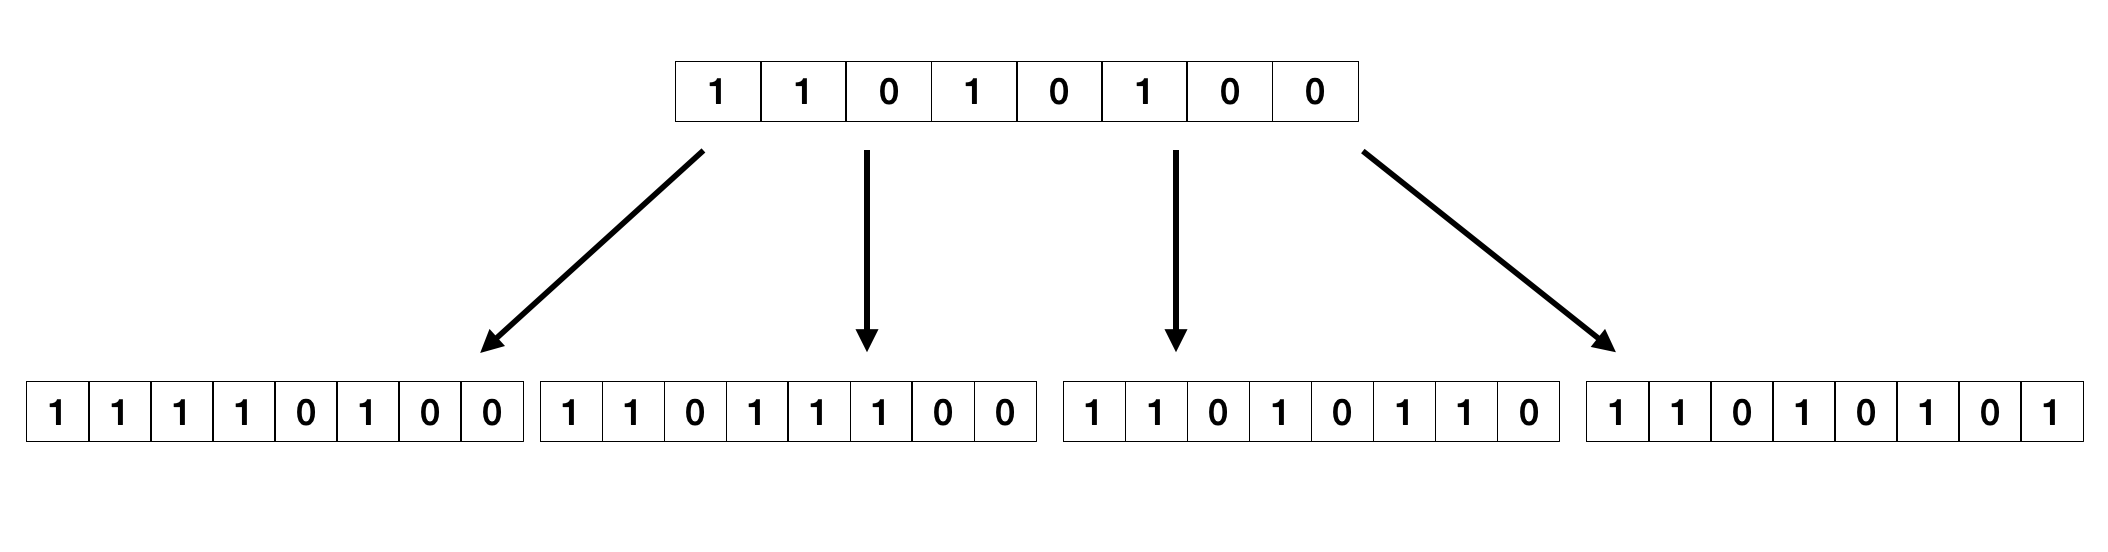
\includegraphics[width=0.95\textwidth]{images/succesores.png}
    \caption{Sucesores de un estado.}
    \label{fig:succ-hillClimbing}
  \end{figure}
  
Finalmente, la función $mejorSuccesor$ se encarga de seleccionar el mejor sucesor de la lista proporcionada.
Para ello, recorre la lista evaluando el valor de la función objetivo $f$ en
cada sucesor y selecciona aquel que tenga el mayor valor (líneas 30 a 38).


%Este enfoque de Hill Climbing presenta la ventaja de tener menos parámetros de configuración que los algoritmos genéticos, 
%lo que simplifica su implementación. Sin embargo, este tipo de búsqueda local implica el riesgo de quedar atrapado en óptimos locales, 
%dado que el algoritmo solo avanza hacia soluciones que mejoran directamente el estado actual. 
%
%En cualquier caso, el enfoque propuesto resulta eficiente en contextos donde se requiere una búsqueda controlada y directa, 
%sin la necesidad de manejar múltiples parámetros adicionales.
%


% En cada iteración, \emph{Hill Climbing} generar los sucesores del estado corriente (Línea 5). Esto se puede observar en el algoritmo \ref{alg:sucessores}. 
% Esto, simplemente, genera estados sucesores prendiendo únicamente un bit (poniendo 1) por cada bit apagado (bit en 0). 
% Esto significa que crear un sucesor para nuestro problema es agregar un método al estado corriente. El método \emph{generarSucesores} nos devuelve el conjunto de estados del estado \emph{curr}. \pp{Esto también está desordenado. Habría que poner un ejemplo con figuras para que se entienda bien qué hace.}

% El método que genera los sucesores nos devuelve un conjunto de posibles soluciones que se crean a partir de sumarle un método a la solución óptima corriente ($curr$). Es decir, los sucesores  $S$ generados con \emph{GenerarSucesores(curr)} de un candidato $curr$ son los conjuntos {$curr\cup{mi}$}, para cada $mi$ $\in$ API (Línea 3) \pp{Se podría poner el pseudocódigo de generar sucesores, y quizás poner un ejemplo para que se entienda}.
% Sea $best$ el sucesor con valor objetivo más alto (línea 6), si este tiene un valor que es menor o igual al corriente, significa que no hay un sucesor mejor y el algoritmo retorna el estado corriente (Línea 7 y 8). Se puede observar que este estado es un máximo local y el algoritmo lo encontró.
% En caso de que el valor del estado corriente sea menor al mejor sucesor encontrado en la iteración, se reemplaza el corriente y vuelve a ejecutar una nueva iteración con este estado hasta encontrar un máximo local. \pp{Esto también está explicado arriba, y ahora de nuevo. Hay que ordenarlo.}
% Observe que $best$ tiene exactamente un método más que el mejor candidato de la iteración anterior, $curr$ (Línea 4) \pp{hay que implementar con código el existe un mejor candidato. Mirar el libro de AI.}.

%Se puede observar que este algoritmo puede quedar atrapado en un máximo local y no generar alguna combinación específica que podría ser aún mejor. Aquí se puede ver que es un algoritmo perezoso, ya que obtiene una solución rápida, pero puede no ser eficaz en encontrar la mejor solución global. 

%\subsubsection{Clases de equivalencia}
%\label{alg:approachCE}
 %Las clases de equivalencia son una técnica utilizada para agrupar conjuntos de datos de entrada en categorías o clases que tienen un comportamiento similar o producen resultados equivalentes. Esta técnica es ampliamente utilizada en el diseño y la realización de pruebas de software.
 %En términos generales, una clase de equivalencia representa  un conjunto de que se espera que produzcan resultados idénticos. La idea es que si un conjunto de la clase de equivalencia produce un resultado, entonces todas las demás entradas de esa clase deberían producir el mismo resultado.
 %Al trabajar con clases de equivalencia, se selecciona una entrada representativa, llamada caso de prueba, de cada clase para ser evaluada. En lugar de probar todas las posibles entradas, se eligen casos de prueba que representen cada clase de equivalencia para minimizar la cantidad total de pruebas necesarias.

 %Bajo esta introducción, hemos desarrollado un tercer algoritmo donde agrupamos en clases de equivalencia aquellos subconjuntos de métodos que tengan el mismo valor de la función objetivo con alguna de las funciones explicadas en \ref{sec:fitness}.

%\subsection{Pseudo-Código}

%\begin{figure}[H]
%\begin{lstlisting}[style=javaStyle, caption={Algoritmo basado en Clases de Equivalencia}, label={algo:clases_equivalencia}]
%public Estado clasesDeEquivalencia() {
%    Estado curr = generarEstadoIncial(problem,funObjectivo);
%    Map<Key, Estado> equivalenceClasses = crearClasesDeEquivalencia(curr);

%    boolean newClassCreated;
%    do {
%        newClassCreated = false;
%        Set<Estados> newCandidates = candidatosPorClase(equivalenceClasses);

%        for (Estado candidate : newCandidates) {
%            Queue<Estado> successors = generarSucesores(candidate);
%            for (Estado successor : successors) {
%                Double key = successor.value;
%                equivalenceClasses.get(key).add(successor);
%                newClassCreated = true;
%            }
%        }
%    } while (newClassCreated);

%    Set<Estado> best = obtenerMejor(equivalenceClasses);
%    return best;
%}
%\end{lstlisting}
%\end{figure}


%En este algoritmo, se comienza obteniendo los conjuntos \emph{singletons} (Línea 1), que son los métodos constructores individuales de la misma manera que el algoritmo de \ref{alg:hill_climbing}. Esto es nuestro estado inicial del algoritmo. A partir de estos singletons, se crea una clase de equivalencia con la \emph{key} que es la función de valoración de cada estado inicial y se agrupan los estados que tienen el mismo valor de valoración. Esto servirá como punto de partida de nuestro algoritmo. (Línea 3).  En el algoritmo las clases de equivalencias están guardadas en $equivalenceClasses$.

%Luego comienza la etapa iterativa (Línea 6 a 18) mientras se haya creado una nueva clase de equivalencia. En cada iteración, se generan nuevos candidatos por cada clase de equivalencia. Es decir, se selecciona un candidato de cada clase de equivalencia (el que tenga menor cantidad de métodos y menor cantidad de parámetros) $candidatosPorClase(equivalenceClasses)$ y se lo guarda en una cola ($newCandidates$) (Línea 8). A continuación, se generan los sucesores (línea 10 y 11) para cada candidato elegido, $GenerarSucesores(candidate)$, utilizando el mismo enfoque que en el algoritmo \ref{alg:sucessores}. Estos se guardan en $successors$. Es decir, si tenemos $N$ clases de equivalencias vamos a tener $N$ candidatos a los cuales le vamos a calcular sus sucesores.  Luego, por cada uno de estos sucesores se le calcula su función de valoración y de acuerdo a esta se lo guarda en la clase de equivalencia representada por el valor de valoración (Línea 14).
%El algoritmo itera hasta que no hayamos creado una nueva clase de equivalencia. Si no hemos creado una clase de equivalencia nueva, quiere decir que no hay cambios y hemos explorado todas las alternativas posibles. 

%Luego, para obtener el mejor conjunto de métodos generadores de objetos que estamos buscando, accedemos a la clase de equivalencia que tenga la \emph{key} más grande (mejor función de valoración) y obteniendo el representante de ese conjunto que tenga menor método y parámetros. Esto lo realiza el método $obtenerMejor(equivalenceClasses)$



% En la búsqueda de soluciones óptimas mediante algoritmos genéticos u otros algoritmos de búsqueda, la función de valoración \cite{goldberg1989genetic} desempeña un papel fundamental. Su diseño adecuado es crucial, ya que determina la dirección y el éxito del proceso de búsqueda.
% La función de valoración evalúa la calidad de cada solución candidata y la compara con otras soluciones en la población. Proporciona una medida objetiva de la idoneidad de cada individuo en relación con los objetivos y restricciones del problema. La calidad se expresa generalmente mediante un valor numérico, donde valores más altos indican soluciones más deseables. Por ejemplo, si estamos resolviendo un problema de optimización en el que buscamos maximizar una función objetivo, la función de valoración puede asignar un valor más alto a las soluciones que se acercan más a la solución óptima. Por otro lado, si estamos resolviendo un problema de minimización, la función de valoración puede asignar un valor más alto a las soluciones que se alejan más de la solución óptima.
% Definir una buena función de valoración implica considerar cuidadosamente los requisitos y características del problema en cuestión. Puede implicar ponderar diferentes objetivos, como maximizar o minimizar ciertas variables, satisfacer restricciones específicas o lograr un equilibrio entre múltiples criterios. 

% Una función de valoración efectiva debe ser capaz de discriminar entre soluciones prometedoras y soluciones subóptimas. Debe proporcionar una evaluación objetiva y precisa, permitiendo la selección de soluciones de alta calidad y la eliminación de soluciones menos deseables.
% Además, la función de valoración debe ser adecuada para el dominio y el tipo de problema abordado. Puede requerir conocimiento especializado y experiencia en el campo para definir correctamente las métricas y ponderaciones apropiadas. 

% Es importante tener en cuenta que la función de valoración puede evolucionar y adaptarse a lo largo del proceso de búsqueda. A medida que el algoritmo de busqueda avanza y produce nuevas generaciones de soluciones, la función de valoración puede ser ajustada y refinada para enfocarse en las características más relevantes y deseadas.


% Por lo tanto, en los algoritmos de búsqueda la función de valoración desempeña un papel crucial para evaluar y comparar soluciones candidatas en función de criterios específicos del problema. Proporciona una medida cuantitativa de la calidad de las soluciones y guía el proceso de selección y toma de decisiones en cada etapa del algoritmo. El diseño adecuado de la función de valoración es esencial para obtener resultados óptimos y eficientes en la resolución de problemas.
% A continuación, explicaremos cada función de valoración implementada en nuestros algoritmos.


% En el caso de algoritmos greedy, la función de valoración juega un papel similar pero con un enfoque más local. En lugar de trabajar con una población de soluciones, los algoritmos greedy toman decisiones en cada paso basándose en una evaluación local de las opciones disponibles. La función de valoración en un algoritmo greedy se utiliza para seleccionar la mejor opción en cada iteración o paso del algoritmo, maximizando o minimizando la función de valoración según el objetivo del problema \cite{cormen2009introduction}.



